\documentclass[a4paper, oneside]{book}

\usepackage{ghilonz}

\title{Fondamenti Matematici per l'Informatica}
\author{Zeno Saletti}
\date{\today}



\begin{document}


\begin{titlepage}
    \newgeometry{left = 0cm, right = 0cm, top = 0cm, bottom = 0cm}
    \pagecolor{blue}\afterpage{\nopagecolor}
    
\includegraphics[width=\textwidth,height=\textheight,keepaspectratio]{bookcoverfmi.pdf}
    \restoregeometry
\end{titlepage}

\chapter*{}

\vspace*{0.3\paperheight}
\begin{center}
    \textbf{Avvertenze!}\\
    Questa è una raccolta di appunti redatta da studenti e
    condivisa per altri studenti. Non pretende di essere un libro
    di testo, ma una forma di aiuto libero e gratuito per coloro
    che fossero in cerca di materiale di supporto allo studio.
    Pertanto, si raccomanda di non preparare l'esame basandosi unicamente
    su questi appunti, ma di fare riferimento alle lezioni frontali
    e ai libri (in breve, a chi è esperto in merito). Qualora quindi
    vi fossero affermazioni fuorvianti o false contenute in queste
    pagine, \textit{gli autori non si assumono la responsabilità di eventuali
    esiti (1) non corrispondenti alle aspettative oppure (2) negativi di esami
    o altre forme di prove ufficiali presso l'Università}; gli autori sono anzi
    aperti a eventuali segnalazioni e correzioni, in primo luogo per colmare lacune di natura concettuale
    nell'esposizione delle nozioni.
\end{center}

\chapter*{Prefazione}

La presente dispensa, tavola di contenuti utili o meno, raccolta di appunti
o qualsivoglia supporto allo studio, nasce come disordinata e incoerente collezione di note
trascritte nel corso delle lezioni, sessioni di studio ed esercitazioni relative al
corso \textit{Fondamenti Matematici per l'Informatica}, durante l'anno accademico
2022/2023 presso l'Università degli Studi di Trento. Evolutasi a raccolta dei teoremi
fondamentali richiesti all'esame, questa dispensa si mostra ora come testo organico e
dignitosamente ordinato. Non si può negare il fatto che fossero già presenti materiali
tramandati da generazioni di studenti durante la stesura di questi appunti, ma sentivamo
forte l'esigenza di riunire in un unico luogo non solo i teoremi, ma anche definizioni,
esempi esplicativi di esercizi d'esame e ulteriori spiegazioni teoriche, talvolta solo
citate oralmente a lezione o difficilmente reperibili.

Ma qui non si discute di mero esercizio formale, di sfoggio di conoscenza o della
presunta padronanza di strumenti tipografici come \LaTeX. Questa dispensa si propone
innanzitutto come risorsa (si spera) utile agli studenti presenti e futuri, del tutto
gratuita. La scienza è umana ed è all'umanità che essa viene messa a disposizione.
In secondo luogo, non è garantita l'assenza di errori, siano essi grammaticali, lessicali,
sintattici, grafici, concettuali, di interpretazione, di conto, distrazioni e così via.
Infine questo testo non pretende, e non potrebbe minimamente farlo, di essere un libro
di testo; perché le nozioni qui mostrate e trascritte non sono altro che il frutto del
lavoro di studenti, non professori o esperti in merito. Nonostante ciò, nell'ordinare
tutti questi appunti è stata prestata la maggior attenzione nel riportare fedelmente il
significato e il pensiero matematico di questa materia straordinaria.

Ultimo, ma forse il più caro tra i motivi che ci hanno spinto a creare queste note, è
la speranza che questo corso appassioni gli studenti di informatica, sia per quanto riguarda
la matematica che per l'informatica stessa, perché l'informatica è progenie della matematica
come la fisica lo è per la filosofia. Certo, molti degli argomenti mostrati sono solo un
assaggio di quel vasto mondo della matematica discreta e per molti sembrerà solo un
conglomerato di concetti astratti, oltre che apparentemente inutili. Ma crediamo nel
seguente postulato

\[ \exists \text{studente}: \text{studente} \in \text{Corso di Informatica}, \text{ studente apprezza la materia} \]

\noindent cioè, crediamo che almeno uno tra i lettori farà tesoro di queste nozioni e che,
come noi, trovi motivo di spingere ancora più in là la propria curiosità, non solo per
l'informatica in sé, ma anche per tutto ciò che ha permesso a questa giovanissima scineza di
progredire, prima fra tutte la matematica.

Non fermatevi solo di fronte alla superficie, perché la totalità del reale non è ancora
stata scoperta a fondo. La tecnica di crittografia RSA, trattata molto brevemente in
queste note, è stata una grande novità e venne sviluppata solamente a partire dagli anni
Settanta del secolo scorso. Finché si ricordava da poco il primo allunaggio, tre persone
pensavano a cosa potevano fare dei semplici numeri interi divisi, moltiplicati, sommati
e sottratti; apparentemente la cosa più banale che si potesse fare. Eppure si fecero
ancora passi avanti in matematica, crittografia e informatica seppur dopo ben 2500 anni
di storia, ovvero dalla trattazione della divisione euclidea, anch'essa citata qui.

Ringraziamo chiunque abbia contribuito, direttamente e indirettamente, a questo progetto:
studenti, con i loro materiali generosamente condivisi e ormai reperibili con gran facilità,
professori, con la chiarezza delle loro lezioni e la disponibilità e l'umorismo, esercitatori,
con i loro segreti sul come passare l'esame. Noi non ci abbiamo messo solo impegno e fatica,
ma curiosità e voglia di saperne ancora di più su questo universo e su noi stessi. Ora tocca
a voi portare avanti la nostra conoscenza, che è la vostra.
\chapter*{Note e Guida al Testo}
Gli argomenti trattati appartengono alla branca della Matematica Discreta,
quindi quella matematica che si occupa non del \textit{continuo} ma di
ciò che è \textit{numerabile} o talvolta \textit{finito}. In parole
semplici, di ciò che si può contare con le dita di una mano. Il corso
è diviso in due parti:
\begin{itemize}
\item \textbf{Aritmetica Modulare:} dalla teoria degli insiemi,
si passerà ai numeri naturali e interi, all'operazione di divisione,
il concetto di congruenza in modulo e infine all'applicazione
del metodo di crittografia RSA.

\item \textbf{Introduzione alla Teoria dei Grafi:} verrà data un'occhiata
ad alcuni grafi, se ne daranno definizioni formali (forse meno familiari
rispetto alla loro controparte grafica) e proprietà rilevanti.
\end{itemize}
In più, vengono aggiunte una terza parte di esercitazione, che riflette
lo schema di lezioni dell'A.A. 2022/2023, ed una quarta che include
alcune appendici.

Questi appunti rispettano ancora fedelmente il loro iniziale mandato:
raccogliere tutti i teoremi utili all'esame, arricchiti con le spiegazioni
e le indicazioni del professore. Per questo li troverete evidenziati
all'interno degli appositi box grigi. Col tempo, si sono aggiunte altre
categorie degne di nota altrettanto evidenziate. Ecco le indicazioni di ogni
colore:
\begin{itemize}
\item \textcolor{gray}{Grigio}: teorema o proposizione rilevante.
\item \textcolor{green}{Verde}: corollario.
\item \textcolor{yellow}{Giallo}: definizione.
\item \textcolor{blue}{Blu}: esempio esplicativo o esercizio con soluzione.
\item \textcolor{red}{Rosso}: nozione utile.
\item \textcolor{violet}{Viola}: il lemma utile.
\end{itemize}
I teoremi richiesti al tempo di stesura sono sottolineati, sia
nei paragrafi che nell'indice, per una veloce consultazione.
Affidarsi all'indice, non solo all'indicazione visiva dei box
grigi.

Si fa qui intenso utilizzo di simboli logico-matematici, sia per
contrarre i predicati e le formule che per produrre fedelmente la
scrittura ideale da adottare all'esame e al di fuori di esso. Si
è posta attenzione, per quanto possibile, ad affiancare a tali
simboli una spiegazione verbale concisa. Sicuramente il testo non
è del tutto privo di abusi di notazione o simbologia non-standard.
Per questi ed altri motivi, \textit{gli apppunti non sostituiscono
interamente le lezioni frontali}. Eventuali spiegazioni più chiare
e precise sono sicuramente fornite, nella stragrande maggioranza dei
casi, dal professore. Questa dispensa mira solo a riassumere i contenuti
delle lezioni.
\chapter*{Errata}
\chapter*{Riconoscimenti}

\section*{Testi}

\section*{Immagini}


%\begin{center}
%    \href{https://github.com/zenosalty/courses-fmi}{Apri una issue su \faGithub \space per cominciare a segnalare errori o miglioramenti.}
%\end{center}

\tableofcontents

\vspace*{2cm}
\begin{center}
    \textbf{Suggerimento:} puoi consultare facilmente questa dispensa
    cliccando sugli elementi dell'indice (a patto che il lettore per
    file \texttt{.pdf} attualmente in uso consenta di usufruire di
    tale funzionalità).
\end{center}


\part{Aritmetica Modulare}

\chptr{Fondamenti di Insiemistica}

\section{Assiomi}
Ai fini del corso, mostriamo solo alcuni assiomi e concetti primitivi,
appartenenti alla teoria degli insiemi, utili a comprendere ciò che
verrà trattato in seguito.

\begin{tcolorbox}[colback = yellow!30, colframe = yellow!30!black, title = {Elemento, insieme, appartenenza}]
Intenderemo \textit{primitivi} i concetti seguenti:
\begin{itemize}
    \item \textbf{Elemento:} intuitivamente, un oggetto qualsiasi.
    \item \textbf{Insieme:} intuitivamente, una collezione di elementi.
\end{itemize}
Un oggetto si può considerare un insieme se è sempre possibile stabilire
\textit{senza ambiguità} se qualcosa è un suo elemento oppure no. Tale
affermazione esprime la relaizone di \textbf{appartenenza} tra elemento e
insieme:
\[ A \text{ è un insieme } \Longleftrightarrow \forall x,x\in A \text{ o}\footnote{Disgiunzione esclusiva: solo una affermazione può e deve essere vera.}\text{ } x\not\in A \]
\end{tcolorbox}

\begin{osservaz}
Un insieme può a sua volta essere un elemento.
\end{osservaz}

\subsection*{Appartenenza e paradosso di Russell}
Anche se la richiesta espressa dalla condizioine di appartenenza può sembrare
scontata, in realtà può essere fonte di problemi. Consideriamo l'oggetto
\[ R = \{x|x\not\in x\} \]
Per capire se $R$ è un insieme, è necessario passare in rassegna ogni oggetto
$x$ e stabilire se esso appartiene o meno a $R$ (affinché $x\in R$, deve valere
la condizione espressa $x\not\in x$). Quando si dice \textit{ogni oggetto} si
intende anche $R$ stesso. Ecco cosa accade quando si tenta di stabilire se
$R\in R$:
\begin{itemize}
\item Se $R\in R$, allora, per costruzione di $R$, deve essere $R\not\in R$.
\item Se invece $R\not\in R$, vuol dire che $R$ non rispetta la condizione, pertanto $R\in R$.
\end{itemize}
Dunque si giunge a concludere che \[ R\in R \Longleftrightarrow R\not\in R \]
che è un'evidente contraddizione. Quello che è stato appena illustrato è il \textit{paradosso
di Russell}\footnote{Per una versione più divertente del paradosso, invitiamo il
lettore a farsi raccontare la favola-paradosso del barbiere. Non ancora soddisfatti? Provate il paradosso del bibliotecario.}. Grazie agli assiomi precedenti, è allora garantito che $R$ non è
un insieme. Un altro esempio di oggetto non classificabile come insieme,
secondo le definizioni presentate finora, è l'\textit{insieme universo} $\mathcal{U}$,
trattato più avanti.

\begin{tcolorbox}[colback=yellow!30, colframe=yellow!30!black, title={Assioma di Estensionalità}]
Due insiemi sono uguali se possiedono gli stessi elementi.
\[ A = B \Longleftrightarrow (\forall x,x\in A \Leftrightarrow x \in B) \]
\end{tcolorbox}

\begin{tcolorbox}[colback=yellow!30, colframe=yellow!30!black, title=Esistenza dell'insieme vuoto]
Esiste un insieme, chiamato insieme vuoto (indicato col simbolo $\varnothing$), che non possiede elementi.
\[\exists \varnothing:\forall x, x\not\in\varnothing\]
Tale insieme è unico (si dimostra attraverso l'Estensionalità).
\end{tcolorbox}

\begin{tcolorbox}[colback=yellow!30, colframe=yellow!30!black, title={Sottoinsiemi}]
Siano $X,Y$ due insiemi. Si dice che $X$ è sottoinsieme di $Y$
(equivalentemente si può dire \emph{è contenuto}), utilizzando il simbolo $\subseteq$,
se ogni elemento di $X$ è elemento di $Y$.
\[ X \subseteq Y \Longleftrightarrow \forall x(x\in X \Rightarrow x\in Y) \]
\end{tcolorbox}

\begin{osservaz}
Esistono molti simboli per indicare i
sottoinsiemi,: $\subset,\subseteq,\subseteqq$.
Si presti bene attenzione a $\subset$: la letteratura
accademica è piuttosto contraddittoria sul significato di tale
simbolo e non è ben chiaro se esso possa essere utilizzato per
indicare unicamente i sottoinsiemi \textbf{propri}, ovvero quelli
che non possono coincidere col sovrainsieme. Per evitare
ambiguità si utilizzano equivalentemente i simboli $\subsetneq,\subsetneqq$, poco usati
qui.
\end{osservaz}

\section{Insiemi e proprietà: l'assioma di separazione}
Un modo di definire alcuni insiemi è quello di impiegare una \textit{proprietà}
che ne caratterizzi gli elementi. Una proprietà non è altro che una proposizione,
cioè un'affermazione vera e propria, come
\[ P(x) := \textit{ x è fan dei Caesars} \]
Ovviamente a noi interesseranno affermazioni relative a oggetti matematici.
In generale $P(x)$ può essere vera o falsa a seconda di $x$, ma asserzioni come
\[ \forall x \quad x\in\varnothing\Longrightarrow P(x) \]
sono sempre vere. Sembra assurdo, ma approfittiamo di questo esempio per
spiegare che il simbolo $\Longrightarrow$ (\textit{se [ipotesi] allora [tesi]}) esprime, in matematica, \textit{l'implicazione logica materiale}.
In altre parole, l'intera implicazione è vera se l'ipotesi è falsa oppure se
è vera la tesi. \textit{Ex falso quodlibet}, dal falso segue ogni cosa. Nel
nostro caso, la tesi $x\in\varnothing$ è sempre falsa, quindi possiamo
supporre che tutti gli elementi dell'insieme vuoto sono fan dei Caesars.


Se $P$ è una proposizione esprimibile
in termini insiemistici, cioè attraverso gli opportuni simboli e connettori
logici, allora scrivendo
\[\{x|P(x)\}\]
si intende la collezione di tutti gli $x$ che soddisfano $P$. Il paradosso
di Russel in realtà è prova che, in generale, un tale oggetto non è
sempre un insieme. Perciò occorre l'assioma della separazione, che tuttavia
non permette di costruire tutti gli insiemi della teoria degli insiemi, i
quali devono essere definiti con altri assiomi
(tali insiemi esulano da questo corso).

\begin{tcolorbox}[colback=yellow!30, colframe=yellow!30!black, title={Assioma della separazione}]
Se $X$ è un insieme e $P$ una proprietà esprimibile come proposizione
scritta in termini del linguaggio della teoria degli insiemi, allora
la collezione
\[ \{x|x\in X, P(x)\} \]
è un insieme. Alternativamente, vale anche la notazione $\{x\in X|P(x)\}$.
\end{tcolorbox}

Possiamo ora spiegare perché non esiste $\mathcal{U}$, l'insieme di tutti
gli insiemi. Supponiamo invece che $\mathcal{U}$ esista; allora possiamo
scrivere
\[ \{x|x\not\in x\} = \{x\in\mathcal{U}|x\not\in x\} \]
Questo perché $x$, nel membro di sinistra, è anche un insieme; dal momento
che $\mathcal{U}$ è un insieme di insiemi, allora $x\in\mathcal{U}$.
Ma per il paradosso di Russell, il primo membro non può essere un insieme;
quello di destra, per l'assioma di separazione, invece lo è, perché abbiamo
supposto l'esistenza di $\mathcal{U}$\footnote{Il paradosso si supera
introducendo la nozione di \textit{classe}, che tuttavia non vedremo qui.}.

\section{Operazioni tra insiemi}
Se $X$ e $Y$ sono insiemi, si possono ricavare altri insiemi, per mezzo
dell'assioma della separazione, attraverso le seguenti operazioni:
\begin{enumerate}
\item \textbf{Intersezione:} $X\cap Y=\{x|x\in X, x\in Y\}$
\item \textbf{Differenza:} $X\setminus Y=\{x|x\in X,x\not\in Y\}$
\item \textbf{Unione:} $X\cup Y=\{x|x\in X \vee x\in Y\}$
\item \textbf{Prodotto:} $X\times Y=\{(x,y)|x\in X, y\in Y\}$
\item \textbf{Potenza:} $2^X=\{x|x\subseteq X\}$
\end{enumerate}
Se $I$ è un insieme e per ogni $i\in I$ è dato un insieme $X_i$
(si dice che gli $X_i$ sono indicizzati su $I$, cioè $I$ serve
solamente a \emph{numerare} o etichettare gli $X_i$), ridefiniamo
unione e intersezione al caso generale di insiemi multipli:
\begin{enumerate}
\item \textbf{Intersezione:} $\bigcap_{i\in I}X_i=\{x|\forall i \quad x\in X_i\}$
\item \textbf{Unione:} $\bigcup_{i\in I}X_i=\{x|\exists i:x\in X_i\}$
\end{enumerate}
A parole, l'intersezione include gli $x$ appartenenti \textit{ad ogni}
$X_i$, mentre l'unione include gli $x$ contenuti in \textit{almeno un}
$X_i$.


\section{Relazioni e funzioni}
\begin{tcolorbox}[colback=yellow!30, colframe=yellow!30!black, title={Relazione}]
Siano $X,Y$ insiemi. Si dice relazione ($\mathcal{R}$) tra $X$ e $Y$ un sottoinsieme
del prodotto tra $X$ e $Y$.
\[\mathcal{R}\subseteq X\times Y\]
Si scriverà anche $x\mathcal{R}y$ per indicare $(x,y)\in\mathcal{R},
\quad x\in X,y\in Y$. Una relazione in $X\times X$, cioè tra $X$ e se stesso,
si chiamerà \textit{relazione binaria} su $X$.
\end{tcolorbox}

Anche nella vita di tutti i giorni, si incontra spesso una classe di relazioni,
dette \textit{relazioni di equivalenza}, che condividono tre proprietà semplici ma per
nulla scontate.

\begin{tcolorbox}[colback=yellow!30, colframe=yellow!30!black, title={Relazione di equivalenza}]
Sia $X$ un insieme e sia $\mathcal{R}$ una relazione binaria su $X$
(cioè $\mathcal{R} \subseteq X \times X$). Diciamo che $\mathcal{R}$ è una
relazione di equivalenza su $X$ se possiede le seguenti proprietà:
\begin{enumerate}
    \item \textbf{Riflessiva:} $\forall x \in X, \quad x \mathcal{R} x$
    \item \textbf{Simmetrica:} $\forall x,y \in X, \quad x \mathcal{R}y \Longrightarrow y \mathcal{R} x$
    \item \textbf{Transitiva:} $\forall x,y,z \in X, \quad x \mathcal{R} y \text{ e } y \mathcal{R} z \Longrightarrow x \mathcal{R} z$
\end{enumerate}
\end{tcolorbox}
La portata di questo genere di relazioni è ampia e copre non solo i linguaggi
matematici, ma anche la logica quotidiana. Ad esempio, qualsiasi cosa è uguale
a sé stessa; se la mia auto ha lo stesso colore della tua, allora la tua auto ha lo stesso
colore della mia; se posso raggiungere Roma in skateboard partendo da Verona,
e posso fare altrettanto da Roma a Foggia, posso viaggiare in skateboard da
Verona a Foggia. In informatica si possono incontrare numerose relazioni di
equivalenza. Generalmente nei corsi di teoria dei linguaggi di programmazione
si tratta \textit{l'equivalenza di tipo}, che è una relazione di equivalenza.
In Java esiste il metodo \texttt{equals} (si occupa del confronto tra oggetti
appartenenti a classi date), la cui definizione deve mandatoriamente
rispettare le proprietà delle relazioni di equivalenza. Tale obbligo spetta
peraltro al programmatore, qualora si decida di effettuare \textit{override}
del metodo.

\begin{tcolorbox}[colback=yellow!30, colframe=yellow!30!black, title={Funzione}]
Una relazione $f\subseteq X\times Y$ si dice \textit{funzione} (o funzione
\textit{totale}) se per ogni $x\in X$ esiste unico $y\in Y$ per cui $xfy$.
\[ f \text{ funzione} \Longleftrightarrow \forall x\in X,\exists!y\in Y:xfy \]
Si scriverà anche $f:X\to Y$ per indicare che $f$ è una funzione (o applicazione)
da $X$ in $Y$ e $y=f(x)$ come sinonimo di $(x,y)\in f$.
\end{tcolorbox}

L'insieme $\{x\in X|\exists y\in Y: y=f(x)\}$ prende il nome di \textit{dominio}
di $f$ ($\text{dom}(f)$), mentre $\{y\in Y|\exists x\in\text{dom}(f):y=f(x)\}$
è l'\textit{immagine} di $f$. In realtà, per la definizione appena data
$\text{dom}(f)=X$, ma ciò è vero per le funzioni \textit{totali}. Esistono
anche funzioni \textit{parziali}, nelle quali per ogni $x\in X$ esiste \textit{al più}
un $y\in Y$ col quale $x$ è in relazione. Per noi saranno importanti le funzioni
totali.

Denotiamo con $Y^X$ l'insieme di tutte le funzioni totali da $X$ a $Y$, cioè
\[ Y^X = \{f\in2^{X\times Y}| \forall x\in X, \exists!y\in Y: xfy\} \]
\begin{osservaz}
Una funzione è interpretabile (come d'altronde accade in fisica) come
una legge che associa ad ogni elemento del dominio $x\in\text{dom}(f)$
uno e un solo elemento del codominio $y\in Y$ tale che $(x,y)\in f$.
Tale elemento è più conosciuto con la notazione $f(x)$. In questo modo,
acquista senso l'uguaglianza $y = f(x)$, che appunto corrisponde a
$(x,y)\in f$.
\end{osservaz}
Se $X$ è un insieme, $\text{id}_X = \{(x_1,x_2\in X\times X| x_1=x_2)\}$ è
una funzione, chiamata \textit{identità} di $X$ e vale \[ \text{id}_X(x)=x \quad \forall x\in X\]
Se $f:X\to Y$ è una funzione e $A\subseteq X$, allora $f\cap(A\times Y)$
è ancora una funzione, chiamata \textit{restrizione di $f$ ad $A$} e indicata
con $f|_A$. In altre parole, essa rappresenta una parte della funzione $f$,
ristretta ad un sottoinsieme del suo dominio.

\begin{tcolorbox}[colback=yellow!30, colframe=yellow!30!black, title={Composizione}]
Siano $f:X\to Y$ e $g:Y\to Z$. Si chiama \textit{composizione}
di $f$ e $g$ la relazione tra $X$ e $Z$ definita da
\[ g\circ f = \{(x,z)| \exists y\in Y: y = f(x) \text{ e } z = g(x)\} \]
\end{tcolorbox}
\begin{osservaz}
Grazie all'osservazione precedente, è possibile scrivere \[ g\circ f = g(f(x)) \]
\end{osservaz}

\begin{tcolorbox}[colback=yellow!30, colframe=yellow!30!black, title={Iniettività, surgettività, bigettività}]
Una funzione $f:X\to Y$ si dice:
\begin{itemize}
    \item \textbf{Iniettiva} se vale: \[ \forall x_1,x_2\in X:x_1 \not= x_2 \Rightarrow f(x_1) \not = f(x_2) \]
    \item \textbf{Surgettiva} se vale: \[ \forall y\in Y, \exists x\in X: f(x) = y \]
    \item \textbf{Bigettiva} se è iniettiva e surgettiva.
\end{itemize}
\end{tcolorbox}

\begin{osservaz}
In una funzione surgettiva, l'immagine coincide con il codominio.
\end{osservaz}




\section{Equipotenza di insiemi}

\chptr{$\mathbb{N}$, Insiemi Ordinati e Insiemi Finiti}

\section{L'insieme $\mathbb{N}$}
Un insieme numerico fondamentale in matematica discreta—in
particolar modo per questo corso—è quello dei numeri naturali,
indicato con il simbolo $\mathbb{N}$. La sua struttura attuale
è dovuta al matematico italiano Giuseppe Peano, che formalizzò
la natura di tale insieme attraverso i suoi celebri assiomi.
\begin{tcolorbox}[colback=yellow!30, colframe=yellow!30!black, title=Assiomi di Peano]
\begin{enumerate}[(i)]
    \item $\mathbb{N}$ ammette almeno un elemento: 0 (zero). \[ 0 \in \mathbb{N} \]
    \item Esiste una funzione iniettiva avente $\mathbb{N}$ come dominio sia come codominio.
    \[ \exists \text{ succ: } \mathbb{N} \rightarrow \mathbb{N} \text{ iniettiva} \]
    \item Il successivo di ogni naturale non è mai 0.
    \[ \forall n \in \mathbb{N}, \text{succ}(n) \not = 0 \]
    \item \textbf{Assioma di induzione:} Se $A\subseteq\mathbb{N}$ è un sottoinsieme contenente 0 e
    per cui vale tale proprietà: per ogni naturale $n$, se $n$ appartiene
    ad $A$, allora anche $\text{succ}(n)$ appartiene ad $A$; allora $A$
    coincide con $\mathbb{N}$.
    \[ [A \subseteq \mathbb{N}: 0 \in A, \quad \forall n \in \mathbb{N} \quad (n \in A \Rightarrow \text{succ}(n) \in A)]  \Longrightarrow  A = \mathbb{N} \]
\end{enumerate}
\end{tcolorbox}

L'assioma di induzione costituisce il principio fondante di
una delle tecniche di dimostrazione più potenti della matematica:
la dimostrazione per induzione. Questa costituirà infatti la
logica di dimostrazione maggiormente sfruttata in questo corso.


\section{Il principio di induzione di prima forma}
\begin{tcolorbox}[title=Prima forma dell'induzione (A)]
Sia $\{P(n)\}_{n \in \mathbb{N}}$ una famiglia di proposizioni
indicizzata su $\mathbb{N}$. Supposto che:
\begin{enumerate}
    \item $P(0)$ sia vera
    \item $\forall n \in \mathbb{N} \quad P(n) \Longrightarrow P(n+1)$
\end{enumerate}
Allora $P(n)$ è vera $\forall n \in \mathbb{N}$.
$\\\\$
\emph{\textbf{Dimostrazione:}} Sia $A = \{n | P(n)\}$. Per la (1) si ha
che $0 \in A$. Se $n \in A$ allora vale $P(n)$, quindi $P(n+1)$
vale per la (2), ma allora $n+1 \in A$, quindi per l'assioma di
induzione $A = \mathbb{N}$.
\cvd
\end{tcolorbox}

Spesso si desidera limitare la dimostrazione di certe proposizioni
ad un sottoinsieme. Per questo esiste una formulazione alternativa
del principio di induzione, utile a tale scopo.

\begin{tcolorbox}[title=Prima forma dell'induzione (B)]
Sia $h \in \mathbb{N}$ e sia $\{P(n)\}_{n \geq h}$ una famiglia
di proposizioni indicizzata su su $n \geq h$. Supposto che:
\begin{enumerate}
    \item $P(h)$ sia vera
    \item $\forall n \geq h \quad P(n) \Longrightarrow P(n+1)$
\end{enumerate}
Allora $P(n)$ è vera $\forall n \geq h$.
$\\\\$
\textbf{\emph{Dimostrazione:}} Sia $A = \{n \geq h| P(n)\}$.

$n=h$ (base dell'induzione) $n=h \Longrightarrow n \in A \because \text{ip. (1)}$.

$\forall n \geq h, n \Rightarrow n+1$ (passo induttivo) Supposto che qualche $n \in A$,
con $n \geq h$ allora per (2) si ha $P(n) \Rightarrow P(n+1)$, ma allora $n+1 \in A$.
Per l'assioma di induzione, $P(n)$ vera $\forall n \geq h$.
\cvd
\end{tcolorbox}

Come per molti altri teoremi che vedremo più avanti, le dimostrazioni del
principio di induzione forniscono uno schema generale per mostrare la validità
di proposizioni indicizzate sui naturali.




\section{Il teorema di ricorsione}
Con i soli assiomi di Peano non si può fare molta strada: non
definiscono operazioni come somma e prodotto e nemmeno relazioni
d'ordine—poter stabilire se un numero è più grande di un altro—
sugli elementi di $\mathbb{N}$. Per poter procedere, è necessario
citare l'assioma di ricorsione—probabilmente il più complesso del
corso, ma sul quale si fondano operazioni scontate come la somma
di numeri naturali.

\begin{tcolorbox}[title=Teorema di ricorsione]
Sia $X$ un insieme, $h:\mathbb{N}\times X\to X$ una funzione
e $c\in X$. Esiste un'unica funzione $f:\mathbb{N}\to X$ tale
che
\begin{align*}
    f(0) &= c\\
    f(\text{succ}(n)) &= h(n,f(n)) \quad \forall n \in\mathbb{N}
\end{align*}

\textit{\textbf{Dimostrazione:}} non vuoi vedere due pagine di dimostrazione
\end{tcolorbox}


\section{Operazioni fondamentali sui naturali}
Enunciato il teorema di ricorsione, definiamo la somma e il prodotto
in $\mathbb{N}$.
\begin{tcolorbox}[colback=yellow!30, colframe=yellow!30!black, title={Somma in $\mathbb{N}$}]
Dato $n\in\mathbb{N}$ si definisce + la funzione $m\mapsto n+m$ ricorsivamente
nel seguente modo:
\begin{align*}
    n + 0 &= n\\
    n + \text{succ}(m) &= \text{succ}(n + m)
\end{align*}
\end{tcolorbox}

Ponendo $\text{succ}(0) = 1$, grazie al teorema di ricorsione si ottiene
\[ \text{succ}(n) = \text{succ}(n + 0) = n + \text{succ}(0) = n + 1 \]
D'ora in poi verrà utilizzata questa scrittura, più naturale e familiare,
per indicare il successivo del numero $n$.

\begin{tcolorbox}[colback=yellow!30, colframe=yellow!30!black, title={Prodotto in $\mathbb{N}$}]
Dato $n\in\mathbb{N}$ si definisce il prodotto $m\mapsto nm$
\begin{align*}
    n0 &= 0\\
    n(m+1) &= nm + n
\end{align*}
\end{tcolorbox}

\begin{osservaz}
Queste definizioni prevedono solo la
somma e il prodotto a sinistra, ma si può mostrare che vale
la \textit{commutatività}, oltre all'associatività e alla
proprietà distributiva.
\end{osservaz}


\section{Insiemi ordinati}
Definita la somma, possiamo tramite essa formalizzare
l'ordinamento dei numeri naturali.

\begin{tcolorbox}[colback=yellow!30, colframe=yellow!30!black, title={Ordinamento in $\mathbb{N}$}]
Siano $n,m\in\mathbb{N}$. Diremo che $n$ è \textit{minore o guale} a $m$
scrivendo
\[ n\leq m \Longleftrightarrow \exists k\in\mathbb{N}: m = n+k \]
\end{tcolorbox}
L'ordinamento sui naturali $\leq$ può essere visto come sottoinsieme
di $\mathbb{N}\times\mathbb{N}$, cioè \[ \leq \quad=\quad \{(n,m)\in\mathbb{N}\times\mathbb{N}|\exists k\in\mathbb{N}:m=n+k\} \]
e dunque $\leq$ è una relazione sui naturali. Infatti $n\leq m$ ha
lo stesso significato di $(n,m)\in\leq$, seguendo la definizione
insiemistica. Valgono poi le seguenti proprietà
(dimostrabili) $\forall n,m,k\in\mathbb{N}$:
\begin{enumerate}
\item $n\leq n$
\item $n\leq m, m\leq n \Longrightarrow n = m$
\item $n\leq m, m\leq k \Longrightarrow n \leq k$
\item $n\leq m \text{ o } m\leq n$
\end{enumerate}

In generale, un ordine degli oggetti può essere stabilito su
quasi tutti gli insiemi. Infatti il linguaggio insiemistico
descrive le regole per tale costruzione estendendole ad un
generico insieme, come si vede nella prossima definizione.
L'ordinamento dei numeri può sembrare qualcosa di totalmente
naturale, ma in realtà e in generale si tratta solo di una
convenzione. In informatica, ad esempio, esiste una relazione
d'ordine sulle stringhe e i singoli caratteri, che si basa
sull'ordine alfabetico di lettere e parole. Nulla vieta di
stabilire ordinamenti su colori o strumenti musicali. Basta
``inventarsi" una relazione sotto forma di proposizione (possibilmente
formale e non ambigua) come ``$x$ viene prima (o con la stessa
priorità) di $y$". Ma come vedremo è necessario stabilire almeno 3 regole
affinche una relazione d'ordine su un certo insieme sia considerabile tale:
\begin{enumerate}
    \item Ogni elemento deve poter essere confrontabile con sé stesso: $x$ viene prima o con la stessa priorità di sé stessp.
    \item Se un elemento è in relazione con un altro, che è in relazione col primo, allora questi elementi sono uguali: se $x$ viene prima o con uguale priorità di $y$ e $y$ viene prima o con uguale priorità di $x$, allora $x = y$.
    \item Se un elemento è in relazione con un altro, che è in relazione con un terzo, allora il primo è in relazione con il terzo: se $x$ viene prima di $y$ e $y$ viene prima di $z$, allora $x$ viene prima di $z$.
\end{enumerate}

\begin{tcolorbox}[colback=yellow!30, colframe=yellow!30!black, title={Relazione d'ordine parziale e totale}]
Sia $X$ un insieme e $\preceq$ una relazione binaria su
$X$. $\preceq$ si dice un ordinamento parziale, o relazione
d'ordine parziale, se valgono se seguenti proprietà:
\begin{enumerate}
    \item \textbf{Riflessiva:} $\forall x\in X \quad x\preceq x$
    \item \textbf{Antisimmetrica:} $\forall x,y\in X \quad x\preceq y, y\preceq x \Longrightarrow x = y$
    \item \textbf{Transitiva:} $\forall x,y,z\in X \quad x\preceq y, y\preceq z \Longrightarrow x\preceq z$
\end{enumerate}
Un ordinamento parziale si dice totale se in più vale la \textbf{tricotomia}
\[ \forall x,y\in X \quad x\preceq y \text{ o } y\preceq x \]
\end{tcolorbox}
Una coppia $(X,\preceq)$ si dice \textit{insieme parzialmente o totalmente
ordinato}.
I simboli (equivalenti) $<,\prec$ indicano l'\textit{ordinamento stretto}, ossia
$x\prec y, x\not=y$. La proprietà di tricotomia può essere riformulata
in termini di ordinamento stretto scrivendo
\[ \forall x,y\in X \text{ vale una e una sola tra } x\prec y \text{ o } x=y \text{ o } y\prec x \]
Introdotto questo nuovo linguaggio, si può allora affermare che
$(\mathbb{N},\leq)$ è un insieme \textit{totalmente} ordinato.

L'ordinamento totale è forse la relazione d'ordine con cui si ha a che
fare più spesso nella vita: i numeri naturali ne sono una dimostrazione
lampante. Ma quindi quando si incontrano relazioni d'ordine \textit{parziali}?
Ma innanzitutto, cosa caspita significa essere una relazione d'ordine totale? Intuitivamente,
una relazione d'ordine totale definita su uncerto insieme permette di
confrontare \textit{sempre} due elementi \textit{qualsiasi} di
quell'insieme. Cioè, se $\mathcal{R}$ è una generica relazione, ad esempio
``è alfabeticamente minore di'' impiegata su un insieme di parole $W$,
il simbolo $x\mathcal{R}y$ ha sempre significato $\forall x,y\in W$.

Un esempio di relazione d'ordine parziale è invece il seguente:
\[ \mathcal{R} = \text{``È antenato di o identico a''} \]
definito sull'insieme degli esseri umani. È facile verificare che
valgono le proprietà (1), (2) e (3) mostrate precedentemente, ma
non vale la tricotomia: non è vero che \textit{per ogni} essere
umano è possibile stabilire se uno è antenato o identico all'altro.
Due fratelli distinti, infatti, non possono essere confrontati con questa
relazione (si ricorda che si è supposto che l'insieme è quello di tutti
gli esseri umani e che la relazione deve valere per tutte le coppie
possibili di elementi; da qui il significato intuitivo del termine
\textit{totale}).

Se il lettore insaziabile desidera una prova dell'utilità di queste
nozioni in ambito informatico, la struttura dati conosciuta come
\textit{heap} definisce un ordinamento parziale sui suoi elementi.
Maggiori informazioni sono disponibili nel corso di \textit{Algoritmi
e Strutture Dati} del famigerato Alberto Montresus\footnote{Personalità
influente presso l'Università di Trento conosciuta anche come Montresor,
Montresorus e altri pseudonimi.}

\section{Insiemi finiti: il lemma dei cassetti}
Forniamo ora una definizione-notazione usata frequentemente in
questo corso: dato un numero naturale $n\in\mathbb{N}$ denotiamo
$I_n = \{0,1,...,n-1\}$. In particolare $I_0 = \varnothing$.

\begin{tcolorbox}[colback=yellow!30, colframe=yellow!30!black, title={Insieme finito}]
Un insieme $X$ si dice finito se esiste un naturale $n$ tale che
$X$ è equipotente a $I_n$. Un insieme è infinito se non è finito.
\[ X \text{ finito} \Longleftrightarrow \exists n\in\mathbb{N}: X\sim I_n \]
\end{tcolorbox}


\begin{tcolorbox}[enhanced, breakable, title={Lemma dei cassetti}]
Siano $X,Y$ due insiemi aventi rispettivamente $X \sim I_n$ e $Y \sim I_m$
con $n < m$. Allora ogni applicazione $f:Y \to X$ non è iniettiva.
$\\\\$
\textit{\textbf{Dimostrazione:}} Si procede per induzione su $n \in
\mathbb{N}$. Se $n=0$ allora $X=\varnothing$ e $Y\not = \varnothing$,
quindi l'insieme $X^Y$ delle applicazioni $Y\to X$ è vuoto e pertanto
non c'è nulla da dimostrare (dal falso segue ogni cosa).

Supponiamo che la tesi sia vera per $n$ e proviamola per $n+1$. Sia
$X \sim I_{n+1}$ e sia $Y \sim I_m$ con $m > n+1$ e supponiamo per
assurdo che l'applicazione $f:Y\to X$ sia iniettiva. Per definizione
esiste una bigezione $g:I_{n+1} \to X$; poniamo $x_n = g(n)$ e
$X' = X-\{x_n\}$. Chiaramente $X'$ è in bigezione con $I_n$. Si
presentano due casi:
\begin{align*}
    f^{-1}(x_n) = \varnothing      &\quad (\text{i.e. }\forall y \in Y: f(y) \not = x_n)\\
    f^{-1}(x_n) \not = \varnothing &\quad (\text{i.e. }\exists y \in Y: f(y) = x_n)
\end{align*}
Nel primo caso, $f(y)\subseteq X'$ e quindi $f:Y\to X'$ sarebbe
un'applicazione iniettiva da un insieme equipotente a $I_m$ in
un insieme equipotente a $I_n$; dato che $m>n+1>n$ questo è assurdo
per ipotesi di induzione.
Nel secondo caso, sia $y\in Y$ tale che $f(y)=x_n$ e sia $Y'=Y-\{y\}$.
Dato che $f$ è iniettiva, $f(Y') \subseteq X'$ e quindi $f|_{Y'}:
Y'\to X'$ è un'applicazione iniettiva. Dato che $Y'\sim I_{m-1}$,
$X'\sim I_n$ e $m-1>n$, ciò è assurdo per ipotesi di induzione.
\cvd
\end{tcolorbox}

Il lemma dei cassetti prende il nome da un modo intuitivo di interpretarlo:
se possiedo un certo numero di oggetti da disporre in un certo numero di
cassetti, più piccolo di quello degli oggetti, allora sicuramente qualche
cassetto conterrà più di un oggetto.
In informatica questo concetto, seppur banale, assume un'importanza da non
sottovalutare: se, in una funzione, si conoscono perfettamente tutti i possibili output e
tutti i possibili input e se questi sono maggiori del numero di output,
allora, per il lemma dei cassetti, almeno un output sarà condiviso da più
input. Ovvero, due o più input produrranno lo stesso output.

\begin{osservaz}
Qualora dominio e codominio abbiano lo stesso numero di elementi,
è possibile per una tale applicazione essere bigettiva, semplicemente
mostrando la sua iniettività. Di fatto il lemma dei cassetti può essere
riformulato come segue: \emph{se n oggetti vengono distribuiti in n posti
cosicché ogni posto non riceva più di un oggetto, allora ogni posto
conterrà uno e un solo oggetto}. Nel teorema di Fermat-Eulero
si farà riferimento a questa formulazione del
lemma dei cassetti.
\end{osservaz}

Dal lemma dei cassetti seguono corollari e definizioni importanti
relativi alle proprietà degli insiemi finiti.
\begin{tcolorbox}[colback=green!30, colframe=green!30!black, title={Equipotenza tra insiemi finiti}]
Dati $n,m\in\mathbb{N}, n\not=m$ e $X,Y$ insiemi finiti tali che $|X|=|I_n|$ e $|Y|=|I_m|$,
allora $X$ e $Y$ non sono equipotenti.

In particolare vale \[ |X|=|I_n|,|X|=|I_m| \Longrightarrow n=m \]
insieme a \[ X\sim I_n,Y\sim I_m \Longrightarrow (X\sim Y \Leftrightarrow n = m) \]
\end{tcolorbox}
Da quest'utlimo corollario si può definire la cardinalità degli insiemi
finiti.

\begin{tcolorbox}[colback=yellow!30, colframe=yellow!30!black, title={Cardinalità di un insieme finito}]
Sia $X$ un insieme finito. Si dice cardinalità di $X$ l'unico numero
naturale $n$ tale che $|X|=|I_n|$. Tale numero si denota con $|X|$.
\end{tcolorbox}

Riproponiamo la condizione di equipotenza, in particolare per quanto
riguarda gli insiemi finiti ed introducendo il linguaggio della cardinalità.

\begin{tcolorbox}[title={Condizione di equipotenza espressa in termini di cardinalità}]
Dati $X,Y$ insiemi finiti vale
\[ X\sim Y \Longleftrightarrow |X|=|Y| \]
\textit{\textbf{Dimostrazione:}} $|X|=|Y|\Longrightarrow \exists n\in\mathbb{N}:
X\sim I_n, Y\sim I_n\Longrightarrow X\sim Y$ per transitività dell'equipotenza.
Viceversa se $X\sim Y$ allora essi hanno la stessa cardinalità, per il
corollario precedente.
\end{tcolorbox}

\begin{tcolorbox}[title={Cardinalità di sottoinsiemi finiti}]
Sia $X$ un insieme finito e $Y\subseteq X$. Allora anche
$Y$ è finito e $|Y|\leq|X|$. Se $Y\subsetneqq X$, allora
$|Y|<|X|$.
\end{tcolorbox}

\begin{tcolorbox}[colback=green!30, colframe=green!30!black, title={Equipotenza tra insieme finito e sottoinsieme}]
Un insieme finito non è equipotente ad alcun suo sottinsieme proprio,
cioè non esiste alcuna bigezione tra $X$ e un qualsivoglia $X'\subsetneqq X$.
\end{tcolorbox}

\begin{osservaz}
Segue in particolare che $\mathbb{N}$ è
infinito. Per gli assiomi di Peano, si può considerare
l'applicazione $n\mapsto \text{succ}(n)$; sapendo che 0 non
possiede alcun predecessore, $\text{succ}$ è una bigezione
tra $\mathbb{N}$ e il suo sottoinsieme proprio $\mathbb{N}\setminus\{0\}$.
$\mathbb{N}$ dunque non soddisfa il corollario precedente.
\end{osservaz}





\section{\underline{Buon ordinamento}}
\begin{tcolorbox}[colback=yellow!30, colframe=yellow!30!black, title=Minimo]
Sia $X$ un insieme e sia $\leq$ un ordinamento su $X$. Sia $A \subseteq X$, diremo
che $z \in A$ è un minimo di $A$ se per ogni $x \in A$ si ha che $z \leq x$.
\[ z = \min A \Longleftrightarrow z \leq x \quad \forall x \in A \]
\end{tcolorbox}

\begin{osservaz}
Non avendo elementi, l'insieme vuoto non ammette minimo.
\end{osservaz}

\begin{tcolorbox}[colback=yellow!30, colframe=yellow!30!black, title=Insieme ben ordinato]
Un ordinamento totale su un insieme $X$ si dice buon ordinamento se ogni sottoinsieme
non vuoto di $X$ ammette minimo.
\[ (X,\leq) \text{ ben ordinato } \Longleftrightarrow \exists \min A \quad \forall A \subseteq X, A \not = \varnothing \]
\end{tcolorbox}

\begin{tcolorbox}[title={Buon ordinamento di $\mathbb{N}$}]
L'ordinamenti dei numeri naturali è un buon ordinamento.
\[ (\mathbb{N},\leq) \text{ ben ordinato} \]
\emph{\textbf{Dimostrazione:}} Sia $A \subseteq \mathbb{N}$ che non
ammette minimo e mostriamo che $A = \varnothing$.
Sia $B = \mathbb{N}\setminus A$ il complementare di $A$. Si procede per induzione su
$n \in \mathbb{N}$ considerando la proposizione:
\[ P(n) := \left(\{0,1,...,n\} \subseteq B\right) \]
$n=0$ (base dell'induzione) Si osservi che $0 = \min\mathbb{N}$, dunque
$0 \not \in A$, altrimenti sarebbe il suo minimo,
allora $0 \in B$ e di conseguenza $\{0\} \subseteq B$.

$n\geq0, n\Longrightarrow n+1$ (passo induttivo)
Supponiamo che $\{0,...,n\} \subseteq B$ per qualche $n\geq0$ (ipotesi
induttiva). Allora
$0,...,n \not \in A$ per ipotesi induttiva, quindi $n+1 \not \in A$,
altrimenti sarebbe il suo minimo. Quindi $n+1 \in B$ e pertanto
$\{0,...,n,n+1\} \subseteq B$. Allora $B = \mathbb{N}$, quindi
$A = \varnothing$.
\cvd
\end{tcolorbox}

Esistono insiemi ordinati ma non ben ordinati? La risposta è affermativa:
\begin{itemize}
    \item $\mathbb{Z}$: il sottoinsieme $M\subseteq \mathbb{Z}$ dei numeri negativi non ha minimo.
    \item $\mathbb{R}$: l'intervallo dei reali $(0,1)$ non ammette minimo.
\end{itemize}




\section{\underline{Il principio di induzione di seconda forma}}
\begin{tcolorbox}[title={Principio di induzione di seconda forma}]
Sia $\{P(n)\}_{n \in \mathbb{N}}$ una famiglia di proposizioni
indicizzate su $\mathbb{N}$ e si supponga che:
\begin{enumerate}
    \item $P(0)$ sia vera
    \item $\forall n > 0 \quad (P(k) \text{ vera } \forall k < n) \Longrightarrow P(n)$
\end{enumerate}
Allora $P(n)$ è vera $\forall n \in \mathbb{N}$.
$\\\\$
\emph{\textbf{Dimostrazione:}} Sia $A := \{n \in \mathbb{N} | P(n) \text{ falsa} \}$,
e si supponga per assurdo che $A \not = \varnothing$. Allora per
la proprietà di buo ordinamento di $\mathbb{N}$, $A$ ammette minimo $m$
(essendo $A\subseteq\mathbb{N}$ non vuoto). Vale:
\[ m := \min A \Longrightarrow m \in A \Longrightarrow P(m) \text{ falsa } \Longrightarrow m \not = 0 \]
che segue da (1).

Se $k \in \mathbb{N}: 0 \leq k < m = \min A$ allora $k \not \in A$. Ma
allora $P(k)$ è vera. Per (2), segue che $P(m)$ è vera, ma si ottiene
così una contraddizione. Deve dunque essere necessariamente $A = \varnothing$,
ovvero $P(n)$ vera $\forall n \in \mathbb{N}$.
\cvd
\end{tcolorbox}
\chptr{$\mathbb{Z}$ e la Divisione}

\section{Qualche parola sui numeri interi}
L'insieme dei numeri interi si denota col simbolo $\mathbb{Z}$
(dal tedesco \textit{Zahl}). Non verrà qui trattata nel dettaglio
la sua struttura, al contrario dei naturali, ma ci limitiamo a
dire che gli interi e le loro operazioni sono definibili per
estensione dai naturali.

\section{\underline{La divisione euclidea}}
\begin{tcolorbox}[enhanced, breakable, title={Teorema della divisione euclidea}]
\[
    n,m \in \mathbb{Z}: m\not=0 \quad \Longrightarrow \quad \exists! q,r\in \mathbb{Z}:
    \begin{cases}
        n = qm + r\\
        0 \leq r < |m|
    \end{cases}
\]
\emph{\textbf{Dimostrazione:}} \underbar{\emph{Esistenza:}} procediamo
per casi. Si consideri dapprima $n,m \in \mathbb{N}$ ($n \geq 0, m > 0$)
e si proceda per induzione, seconda forma, su $n\in\mathbb{N}$.

Se $n = 0$ (base dell'induzione) è sufficiente prendere $q = 0 = r$. Il
sistema della tesi è infatti soddisfatto.

Si supponga ora che $n > 0$ e che la tesi sia vera $\forall k < n$.
Se $n < m$ basta prendere $q = 0$ e $r = n$ (anche qui le condizioni
del sistema sono soddisfatte). Altrimenti si ponga $k = n - m$, dato
che $m > 0$ e pertanto si ha $0 \leq k < n$,
quindi per ipotesi induttiva $\exists q,r \in \mathbb{Z}$ tali che:
\[ 
    \begin{cases}
        k = qm + r\\
        0 \leq r < m = |m|
    \end{cases}
\]
Ma allora $n = k + m = qm + r + m = (q+1)m + r$ e il passo induttivo
è verificato.

Si consideri ora il caso $n < 0$ e $m > 0$. Allora $-n > 0$ e quindi
per il caso precedente esistono $q,r \in \mathbb{Z}$ tali che
$-n = qm + r$ e $0 \leq r < m = |m|$. Per ricondurci alla forma della
tesi, si pone $n = (-q)m - r$. Per sistemare $r$, nel caso $r = 0$ si
soddisfano le condizioni per raggiungere la tesi, se $0 < r < m$ allora
$0 < m - r < m = |m|$ ($m - r$ è pertanto il resto cercato) e:
\[ n = (-q)m - r = (-q)m - m + m - r = (-q - 1)m + (m - r) \]
Infine, se $m < 0$ allora $-m > 0$, quindi per i due casi precedenti
$\exists q,r \in \mathbb{Z}$ tali che:
\[ n = q(-m) + r = (-q)m + r \qquad \text{con } 0 \leq r < -m = |m| \]
\underbar{\emph{Unicità:}} supponiamo che
$qm + r = n = q'm + r'$ e che, a meno di scambiare $r$ e $r'$, $0 \leq r,r' < |m|$.
Supponiamo che $r' \geq r$, allora:
\[ qm + r = q'm + r' \Longleftrightarrow (q - q')m = r'-r \]
\[ \therefore \]
\[ |q-q'||m| = |r'-r| = r'-r < |m| \Longleftrightarrow 0 \leq |q-q'| < 1 \]
Ma dal momento che $q,q' \in \mathbb{Z}$:
\[
    |q-q'| = 0 \Longleftrightarrow q = q' \quad \Longrightarrow \quad qm + r = q'm + r' \Longrightarrow r = r'
\]

\cvd
\end{tcolorbox}

La dimostrazione del teorema costituisce il procedimento alla base
dell'algoritmo ricorsivo per il calcolo del quoziente e del resto
della divisione intera.
\begin{tcolorbox}[enhanced, breakable, colback=red!30, colframe=red!30!black, title=Algoritmo di divisione euclidea]

\end{tcolorbox}

\section{\underline{Rappresentazione dei naturali in base} $b$}
\begin{tcolorbox}[colback=yellow!30, colframe=yellow!30!black, title=Rappresentabilità dei naturali in base arbitraria]
Sia $b\in\mathbb{N}$. Diremo che $n\in\mathbb{N}$ è rappresentabile in base $b$ se
esistono $\varepsilon_0,...,\varepsilon_k\in I_b=\{0,...,b-1\}$ tali che:
\[ n=\varepsilon_0b^0+...+\varepsilon_k b^k = \sum_{i=0}^{k}\varepsilon_ib^i \]
\end{tcolorbox}

\begin{osservaz}
È importante notare che nessun numero è rappresentabile in base 0, perché
$I_0 = \varnothing$ e dunque non esistono simboli che possono rappresentare
i numeri. L'unico naturale rappresentabile in base 1 è 0.
\end{osservaz}

La rappresentabilità è esprimibile in maniera alternativa, come si vede dall'enunciato
del seguente teorema:

\begin{tcolorbox}[enhanced, breakable, title={Teorema di rappresentazione dei naturali in base arbitraria}]
Sia $b \in \mathbb{N}:b \geq 2$. Allora ogni
$n \in \mathbb{N}$ è rappresentabile univocamente nella base $b$.
Ossia esiste una successione $\{\varepsilon_i\}_{i \in \mathbb{N}}$:
\begin{enumerate}
    \item definitivamente nulla ($\exists i_0 \in \mathbb{N}: \varepsilon_i = 0 \quad \forall i > i_0$)
    \item $\varepsilon_i \in I_b \quad \forall i \in \mathbb{N}$ ($0 \leq \varepsilon_i < b$, di tipo resto)
    \item $n = \sum_{i = 0}^{\infty} \varepsilon_i b^i$ (per la (1) tale serie è finita)
\end{enumerate}
e se $\{\varepsilon'_i\}_{i \in \mathbb{N}}$ è un'altra
successione che soddisfa gli stessi punti, allora $\varepsilon_i =
\varepsilon'_i \quad \forall i \in \mathbb{N}$.
$\\\\$
\emph{\textbf{Dimostrazione:}} Sia fissato $b\in\mathbb{N}:b\geq2$.

\underbar{\emph{Esistenza:}} Si procede per induzione, seconda forma, su $n \in \mathbb{N}$.

Se $n = 0$ basta scegliere una successione tale che $\varepsilon_i = 0 \quad \forall i \in \mathbb{N}$.

Assumiamo ora $n > 0$ e si supponga che la tesi sia vera $\forall k < n$.
Si consideri la divisione euclidea tra $n,b$: siano $q,r$ tali che $n = qb + r$
con $0 \leq r < b$. Essendo inoltre $b \geq 2$ vale: $0 \leq q < qb \leq qb + r = n$
e quindi, per ipotesi di induzione, eiste una successione definitivamente
nulla $\{\delta_i\}$ costituita di interi tali che
$0 \leq \delta_i < b \quad \forall i$
e tale che $q = \sum_{i=0}^{\infty}\delta_i b^i$. Segue che:

\[ n = qb + r = \left(\sum_{i=0}^{\infty}\delta_i b^i\right)b + r = \sum_{i=0}^{\infty}\delta_i b^{i+1} + r = \sum_{j=1}^{\infty} \delta_{j-1}b^j + \varepsilon_0 = \sum_{i=0}^{\infty}\varepsilon_i b^i \]

(Si noti che si è posto $\varepsilon_0 = \varepsilon_0 b^0 = r$ e
$\varepsilon_i = \delta_{j-1} \quad \forall i,j > 0$).
La successione $\{\varepsilon_i\}$ è definitivamente nulla, essendo
tale $\{\delta_i\}$ e inoltre $0 \leq \varepsilon_i = \delta_{j-1} < b
\quad \forall i,j > 0$ e $0 \leq \varepsilon_0 = r < b$.
$\newline$
\underbar{\emph{Unicità:}} Si procede per induzione su $n \in \mathbb{N}$.

Se $n = 0 = \sum_{i} \varepsilon_i b^i$ allora ogni addendo della somma,
essendo non negativo ($b \geq 2, \varepsilon_i \in I_b \quad \forall i$), necessariamente deve essere nullo, pertando si
ha $\varepsilon_i = 0 \quad \forall i$.

Si assuma ora $n > 0$ e si suppanga che, $\forall k < n$, l'espressione
in base $b$ sia unica. Sia $n$ tale che:
\[
    n = \sum_{i=0}^{\infty}\varepsilon_i b^i = \sum_{i=0}^{\infty}\varepsilon'_i b^i \Longrightarrow
    n = \left(\sum_{i=1}^{\infty}\varepsilon_i b^{i-1}\right)b + \varepsilon_0 = \left(\sum_{i=1}^{\infty}\varepsilon'_i b^{i-1}\right)b + \varepsilon'_0
\]
Per l'unicità della divisione euclidea, si ha che $\varepsilon_0 = \varepsilon'_0$
e $\sum_{i=1}^{\infty}\varepsilon_i b^{i-1} = q = \sum_{i=1}^{\infty}\varepsilon'_i b^{i-1}$.
Vale $q < n$ (si veda l'esistenza) e pertanto, per ipotesi di induzione,
$\varepsilon_i = \varepsilon'_i \quad \forall i \geq 1$.
\cvd
\end{tcolorbox}
In informatica si incontrano spesso numeri rappresentati in basi
diverse da quella decimale, in modo particolare binaria, ottale
ed esadecimale. Tutto questo è possibile perché il teorema precedente
lo garantisce, sia nella capacità di rappresentare i numeri che
nell'unicità di tali rappresentazioni.

Come per la divisione euclidea, la dimostrazione di questo teorema
mostra un procedimento ricorsivo per il calcolo della stringa che
rappresenta il numero naturale preso in esame data una certa base.

\begin{tcolorbox}[enhanced, breakable, colback=red!30, colframe=red!30!black, title = {Algoritmo di conversione tra rappresentabilità dei naturali in basi diverse}]

\end{tcolorbox}


\section{Proprietà della divisibilità in $\mathbb{Z}$}
Finora abbiamo incontrato la nozione di \textit{divisione}
attraverso quella euclidea, che tuttavia può dare origine
al cosiddetto resto $r$. Un caso interessante di questo
tipo di divisione è proprio quello in cui risulta $r = 0$:
intuitivamente, qualora il divisore ``ci sta esattamente un certo numero
(intero) di volte'' nel dividendo. Questo è il concetto di
\textit{divisibilità} in $\mathbb{Z}$, di cui introduciamo ora la definizione
formale.

\begin{tcolorbox}[colback=yellow!30, colframe=yellow!30!black, title=Divisibilità]
Dati $n,m \in \mathbb{Z}$ si dice che $n$ è un divisore di
$m$ (o che $m$ è un multiplo di $n$) se esiste un $k \in \mathbb{Z}$
tale che $m = kn$:
\[ n|m \quad \Longleftrightarrow \quad \exists k \in \mathbb{Z}: m = kn\]
\end{tcolorbox}

\begin{osservaz}
Dalla definizione valgono le seguenti:
\begin{enumerate}
    \item $n|0 \quad \forall n \in \mathbb{Z}$
    \item $n \not = 0 \Longrightarrow 0 \not | n$
    \item $0|0$
    \item $\pm 1 | n$, $\pm n|n \qquad \forall n \in \mathbb{Z}$
\end{enumerate}
\end{osservaz}

\begin{tcolorbox}[title={Proprietà della divisibilità}]
Dati $n,m\in\mathbb{Z}$ valgono
\begin{enumerate}
    \item $n|m$, $m|q \Longrightarrow n|q$
    \item $n|m$, $m|n \Longrightarrow n = \pm m$
\end{enumerate}
\textit{\textbf{Dimostrazione:}}
\begin{enumerate}
    \item $n|m \Rightarrow m = kn$, $m|q \Rightarrow q = hm = (hk)n \Longrightarrow n|q$
    \item $n|m \Rightarrow m = kn$, $m|n \Rightarrow n = hm \Longrightarrow m = khm \Longleftrightarrow m(1-kh) = 0 \quad \therefore \quad$ $m = 0, n = 0 \because n = hm$ oppure
    $1 - kh = 0 \Longrightarrow h = k = \pm 1 \therefore n = \pm m$
\end{enumerate}
\cvd
\end{tcolorbox}

\begin{tcolorbox}[colback=violet!30, colframe=violet!30!black, title={Lemma utile}]
Siano $c,n,m\in\mathbb{Z}:c|n,c|m$. Allora $c$ divide ogni combinazione lineare
in $\mathbb{Z}$ tra $n$ e $m$:
\[ c|xn+ym \quad \forall x,y\in\mathbb{Z} \]
\textit{\textbf{Dimostrazione:}}

\begin{align*}
    c|n,c|m \Rightarrow&\\
    \Rightarrow &\exists h,k\in\mathbb{Z}:n=ch,m=ck \Rightarrow\\
    \Rightarrow &xn+ym=xch+yck=c(xh+yk) \Rightarrow\\
    \Rightarrow &c|xn+ym
\end{align*}

\cvd
\end{tcolorbox}


\section{\underline{Definizione, esistenza e unicità del MCD}}
\begin{tcolorbox}[colback=yellow!30, colframe=yellow!30!black, title=Massimo Comun Divisore]
Dati $n,m \in \mathbb{Z}$ non entrambi nulli e $c\in\mathbb{Z}$, si dice che
$M = (n,m)$ è \textit{il} massimo comun divisore di $n$ e $m$ se:
\begin{enumerate}
    \item $M>0$
    \item $M|n$ e $M|m$
    \item $\forall c\in\mathbb{Z}:c|n, c|m \Longrightarrow c|M$
\end{enumerate}
\end{tcolorbox}
\begin{tcolorbox}[title={Esistenza e unicità del massimo comun divisore}]
Dati $n,m \in \mathbb{Z}$ non entrambi nulli eiste unico il loro
massimo comun divisore: \[ n,m \in \mathbb{Z}: n \not = 0 \vee m \not = 0 \Longrightarrow \exists! M = (n,m) \]
\emph{\textbf{Dimostrazione:}} \underbar{\emph{Esistenza:}} Si consideri l'insieme
\[S := \{s \in \mathbb{Z}| s > 0, \exists x,y \in \mathbb{Z}: s = xn + ym\}\]
Possiamo asserire che $S \not = \varnothing$, perché vale $nn + mm > 0$
(si ricorda che $n,m$ non sono entrambi nulli). Poiché $S$ è un sottoinsieme non vuoto
di $\mathbb{N}$, grazie al teorema del buon ordinamento di $\mathbb{N}$, $S$
ammette minimo. Sia $d:= \min S = xn + ym$, per qualche $x,y\in\mathbb{Z}$ e dimostriamo che
$d$ è il MCD. Vale $d\in S\Longrightarrow d>0$ (definizione (1)). Sia \[ c\in\mathbb{Z}:
c|n,c|m \Longleftrightarrow \exists h,k\in\mathbb{Z}:n=kc,m=hc \Longrightarrow d=xkc+yhc=(xk+yh)c \Longrightarrow c|d \]
(definizione (2)).  Dimostriamo che $d|n$.
Si consideri la divisione euclidea tra $n$ e $d$: $n = qd + r$ con
$0 \leq r < d$. Se $r > 0$, allora $r = n - qd = n - q(xn + ym) = n(1-qx) +
m(-qy) \in S$. Ma questo è assurdo, perché $r<d$ e $d = \min S$. Quindi
$r=0$ cioè $d|n$. Lo stesso ragionamento vale per $d|m$ (definizione (3)).

\underbar{\emph{Unicità:}} Supponiamo che $M,M'$ siano due massimi comun
divisori di $n,m$. Allora $M'|M$, perché $M|n,M|m$, essendo $M$ divisore
comune. Ma invertendo i ruoli vale anche $M|M'$, perché anche $M$ si
suppone essere massimo comun divisore. Per la proprietà della divisibilità,
allora $M = \pm M'$, ma essendo entrambi i massimi comun divisori di $n$
e $m$, per definizione $M,M'>0$, quindi $M=M'$.
\cvd
\end{tcolorbox}
Dalla dimostrazione segue che, dati $n,m\in\mathbb{Z}$, esistono
$x,y\in\mathbb{Z}$ tali che \[ (n,m) = nx + my \]
e che gli interi che sono combinazione lineare di $n$ e $m$ sono       
tutti e soli multipli di $(n,m)$. È altresì importante notare che:
\begin{enumerate}
\item La nozione di divisibilità non dipende dai segni:
\begin{align*}
    &n|m \Longleftrightarrow \exists k\in\mathbb{Z}:m=kn \Longleftrightarrow \exists k\in\mathbb{Z}:m=(-k)(-n) \Longleftrightarrow -n|m\\
    &\Longleftrightarrow\\
    &\exists k\in\mathbb{Z}:-m=(-k)n=k(-n) \Longleftrightarrow n|-m,-n|-m\\
    &\Longleftrightarrow\\
    &(n,m) = (-n,m) = (-n,-m) = (|n|,|m|)
\end{align*}
\item La definizione di massimo comun divisore non dipende dall'ordine
di $n$ e $m$: \[ (n,m)=(m,n) \]
\item Siano $n,m\in\mathbb{Z}$ non entrambi nulli. Allora
\[ (n,m)=\max\{c\in\mathbb{Z}| c|n,c|m\} \]
\item Sia $n\in\mathbb{Z}\setminus\{0\}$. Vale \[ (n,0)=|n| \]
\end{enumerate}



\section{Algoritmo di Euclide per il calcolo del MCD}
\begin{tcolorbox}[title=Algoritmo di Euclide]
Siano:
\begin{enumerate}
    \item $n,m \in \mathbb{Z}$
    \item $n = qm + r$ la divisione euclidea di $n$ per $m$
    \item $\mathcal{A} := \{c \in \mathbb{Z}| c|n, c|m\}$, $\mathcal{B} := \{c\in \mathbb{Z}| c|m, c|r\}$
\end{enumerate}
Allora $\mathcal{A} = \mathcal{B}$ e in particolare $(n,m) = (m,r)$.
$\\\\$
\emph{\textbf{Dimostrazione:}} mostriamo che $\mathcal{A}\subseteq\mathcal{B}$.
Sia $c\in\mathcal{A}$. Vale:
\[ c\in\mathcal{A} \Leftrightarrow c|n,c|m \Leftrightarrow \exists h,k\in\mathbb{Z}:n=hc,m=kc \Rightarrow r=n-qm=hc-qkc=(h-qk)c \Rightarrow c|r \Rightarrow c\in\mathcal{B} \]

Mostriamo che $\mathcal{B}\subseteq\mathcal{A}$. Sia $c \in \mathcal{B}$. Vale:
\[ c\in\mathcal{B} \Leftrightarrow c|m,c|r \Leftrightarrow \exists h,k\in\mathbb{Z}:m=hc,r=kc \Rightarrow n=qm+r=qhc+kc=(qh+k)c \Rightarrow c|n \Rightarrow c\in\mathcal{A} \]

Segue che \[ \mathcal{A}\subseteq\mathcal{B},\mathcal{B}\subseteq\mathcal{A}\Longrightarrow\mathcal{A}=\mathcal{B} \]

In particolare, per il teorema di esistenza e unicità del MCD e l'Osservazione
(3) di questa sezione, segue che $(n,m) = \max \mathcal{A} = \max \mathcal{B} = (m,r)$.
\cvd
\end{tcolorbox}

\begin{tcolorbox}[colback=red!30, colframe=red!30!black, title=Impiegare l'Algoritmo di Euclide]

\end{tcolorbox}


\section{Numeri coprimi e primi}
\begin{tcolorbox}[colback=yellow!30, colframe=yellow!30!black, title=Numeri coprimi]
$n,m \in \mathbb{Z}$ non entrambi nulli si dicono coprimi se vale:
\[(n,m)=1\]
\end{tcolorbox}
\begin{osservaz}
\emph{$(n,m) = 1 \Longleftrightarrow \exists x,y \in \mathbb{Z}:
nx + my = 1$. In particolare, $(n,n+1)=1$; infatti $1 = (n+1)1 + n(-1)$.}
\end{osservaz}
Avendo introdotto il massimo comun divisore, è ora possibile mostrare
una loro proprietà che permette di metterli in relazione con i
numeri coprimi. Siano infatti $n,m\in\mathbb{Z}$ non entrambi nulli.
Vale allora \[ \left(\frac{n}{(n,m)},\frac{m}{(n,m)}\right) = 1 \]
ovvero, dividendo $n$ e $m$ per il loro massimo comun divisore, si ottengono
numeri tra loro coprimi. La dimostrazione è la seguente:
\[ d = (n,m) \Longleftrightarrow \exists x,y\in\mathbb{Z}: d = nx + my \therefore \frac{d}{d} = \frac{nx+my}{d} \Longleftrightarrow 1 = \frac{n}{d}x + \frac{m}{d}y \]
\cvd

\begin{tcolorbox}[colback=yellow!30, colframe=yellow!30!black, title=Numero primo]
Il numero $p \geq 2$ si dice primo se i suoi unici divisori sono $\pm 1, \pm p$.
\[ p \text{ primo} \Longleftrightarrow \nexists c\in\mathbb{Z}, c\not=\pm1, c\not=\pm p: c|p, \quad p\geq2 \]
\end{tcolorbox}

I numeri coprimi godono di alcune proprietà che verranno sfruttate
in dimostrazioni successive. Siano $n,m,q\in\mathbb{Z}$ con $n,m$
non entrambi nulli. Valgono:
\begin{enumerate}
\item $(n,m) = 1 \text{ e } n|mq \Longrightarrow n|q$
\item $(n,m) = 1 \text{ e } n|q \text{ e } m|q \Longrightarrow nm|q$
\end{enumerate}
\textit{\textbf{Dimostrazione:}}
\begin{enumerate}
\item $(n,m)=1\Rightarrow\exists x,y\in\mathbb{Z}:(n,m)=xn+ym=1\Rightarrow q=qxn+qym\Rightarrow n|mq\Rightarrow\exists h\in\mathbb{Z}:mq=nh\Rightarrow q=qxn+ynh = n(qx+yh)\Rightarrow n|q$
\item $n|q\Rightarrow\exists h\in\mathbb{Z}:q=nh \quad\Rightarrow\quad m|q=nh, (n,m)=1\stackrel{\text{(1)}}{\Longrightarrow} m|h \Rightarrow\exists k\in\mathbb{Z}:h=km\Rightarrow q=nh=nmk\Rightarrow nm|q$
\end{enumerate}
\cvd

\begin{tcolorbox}[colback=green!30, colframe=green!30!black, title=Condizione alternativa di primalità]
\[ p \text{ primo} \Longleftrightarrow \forall n,m\in\mathbb{Z}:(p|nm\Rightarrow p|n \text{ o } p|m) \]
\end{tcolorbox}

Citiamo un'ulteriore proprietà sui numeri primi, della quale si
farà menzione più avanti.

\[ n_1,n_2,\dots,n_k\in\mathbb{Z}, p \text{ primo}: p|n_1n_2\dots n_k \Longrightarrow \exists i\in\{1,\dots,k\}:p|n_i \]
    


\section{\underline{Definizione, esistenza e unicità del mcm}}
\begin{tcolorbox}[colback=yellow!30, colframe=yellow!30!black, title=Minimo Comune Multiplo]
Siano $n,m \in \mathbb{Z}$. Un numero intero $M$ è il minimo
comune multiplo tra $n$ e $m$ se:
\begin{enumerate}
    \item $M \geq 0$
    \item $n|M$ e $m|M$
    \item $\forall c \in \mathbb{Z}: n|c, m|c \Longrightarrow M|c$
\end{enumerate}
Si utilizzerà il simbolo $[n,m]$ per indicare tale $M$.
\end{tcolorbox}


\begin{tcolorbox}[title={Esistenza e Unicità del Minimo Comune Multiplo}]
Dati $n,m\in\mathbb{Z}$, esiste unico il loro minimo comune multiplo:
\[ n,m \in \mathbb{Z} \Longrightarrow \exists!M=[n,m] \]
Nota: $n = m = 0 \Longrightarrow [n,m] = 0$. Per $n,m$ non entrambi nulli:
$[n,m] = \frac{nm}{(n,m)}$
$\\\\$
\emph{\textbf{Dimostrazione:}} \underline{\textit{Esistenza}}
L'unico multiplo di 0 è sé stesso, dunque se $n=0=m$ basta porre
$[n,m]=0$. Sia $M = \frac{nm}{(n,m)} = n'm'(n,m)$. Si è posto $n = n'(n,m)$ e
$m = m'(n,m)$. Segue che: $M = nm' = n'm$ e allora $n|M$ e $m|M$.

Sia $c\in\mathbb{Z}:n|c,m|c$. Allora $(n,m)|c$
\footnote{Per definizione $(n,m)|n,(n,m)|m \Rightarrow \exists h,k\in\mathbb{Z}:n=h(n,m),m=k(n,m)$.
Quindi se esiste $c$ tale che $n|c,m|c$ allora $c=in=i(n,m),c=jm=jk(n,m)$ per qualche $i,j\in\mathbb{Z}$.
Dunque $(n,m)|c$.}.
Ponendo $c = c'(n,m)$ segue $n'|c'$ e $m'|c'$. Essendo $(n',m')=1$ per
proprietà dei coprimi, grazie ancora alle proprietà dei coprimi $n'm'|c'$
quindi
\[M = n'm'(n,m)| c'(n,m) = c\]

\underline{\textit{Unicità:}} Supponiamo che $M,M' \in \mathbb{Z}$
siano due minimi comuni multipli per $n,m$. Da (2) e (3) della
definizione segue che $M|M'$ ma anche, scambiando i ruoli, $M'|M$.
Ma allora, per la proprietà della divisibilità, deve essere
$M = \pm M'$. Ma per (1) della definizione necessariamente segue
che $M = M'$.
\cvd
\end{tcolorbox}

\section{\underline{Teorema fondamentale dell'aritmetica}}
\begin{tcolorbox}[enhanced, breakable, title={Teorema Fondamentale dell'Aritmetica}]
Ogni naturale $n \geq 2$ può essere fattorizzato in numeri primi (positivi),
ovvero può essere scritto come prodotto di numeri primi eventualmente ripetuti:
\[n = p_1p_2 \dots p_a  \quad (a \geq 1 \text{ e } p_i \text{ primo}) \]
Inoltre questa scrittura è unica a meno di riordinamento, ovvero: se
$n = q_1 \dots q_b$, dove $q_j$ con $1\leq j \leq b$ sono primi, allora esiste
una bigezione $\varphi: \{1,...,a\} \to \{1,...,b\}$ tale che
$q_j = p_{\varphi(j)}$.
$\\\\$
\emph{\textbf{Dimostrazione:}} \underbar{\emph{Esistenza:}} Si procede per induzione di seconda
forma su $n \geq 2$, considerando la proposizione $P(n) = $ "il numero naturale $n$ si può scrivere
$n = p_1...p_a$ per qualche $p_1,...,p_a$ primi eventualmente ripetuti".

$n = 2$ (base): $n = 2$ è un numero primo, quindi $a = 1$, $p_1 = n = 2$, quindi
$n = p_1 = 2$.

$n > 2, \forall 2 \leq k < n \Rightarrow n$ (passo induttivo): sia $n > 2$.
Assumiamo di saper scrivere ciascun $2\leq k < n$ come
prodotto di numeri primi eventualmente ripetuti (ipotesi induttiva). Dobbiamo
provare che anche $n$ ammette una tale fattorizzazione. Se $n$ è primo, allora
$a = 1$ e $p_1 = n$, quindi $n = p_1$. Supponiamo che $n$ non sia primo, allora
$n = d_1d_2$ con $2 \leq d_1,d_2 < n$, quindi per ipotesi induttiva $d_1 = p_1...p_a$
e $d_2 = q_1...q_b$ ($a,b\geq1$ con $p_1,...,p_a,q_1,...,q_b$ numeri primi eventualmente
ripetuti). Ma allora $n = d_1d_2 = p_1...p_aq_1...q_b$.

\underbar{\emph{Unicità:}} Supponiamo che esista $n \geq 2$ con due fattorizzazioni:
$n = p_1...p_a = q_1...q_b$ per qualche $p_1,...,p_a$, $q_1,...,q_b$ primi
eventualmente ripetuti. Dobbiamo provare che $a=b$ e $p_i = q_i \quad \forall
i \in \{1,...,a\}$ a meno di riordinamento. Osserviamo che $a \leq b$. Si
procede per induzione (prima forma) su $a \geq 1$ considerando $P(a) =$ "per
ogni $b \geq a$, per ogni $p_1,...,p_a,q_1,...,q_b$ primi tali che $p_1...p_a = q_1...q_b$;
allora $a=b$ e, a meno di riordinamento, $p_i = q_i \quad \forall i \in \{1,...,a\}$".

$a=1$ (base) Sia $b \geq 1$ e siano $p_1,q_1,...,q_b$ numeri primi tali che
$p_1 = q_1...q_b$. Dobbiamo provare che $b=1$ e $p_1 = q_1$. Supponiamo per
assurdo che $b \geq 2$. Vale: $p_1 = q_1(q_2...q_b)$, cioè $q_1|p_1$. Ma dal
momento che essi sono numeri primi, deve essere $p_1 = q_1$,
ma qindi $1 = q_2...q_b$, che è assurdo.

$a \geq 1, a \Rightarrow a+1$ (passo induttivo) Supponiamo che vengano dati $p_1,...,p_a,
q_1,...,q_b$ numeri primi con $b \geq a$ e $p_1...p_a = q_1...q_b$. Allora
assumiamo che $a=b$ e, a meno di riordinamento, $p_i = q_i \quad \forall i \in \{1,...,a\}$
(ipotesi induttiva). Dobbiamo dimostrare che: $P(a+1)= $"sia $b \geq a+1$ e siano
$p_1,...,p_{a+1},q_1,...,q_b$ primi tali che $p_1...p_{a+1} = q_1...q_b$.
Allora $b = a+1$ e $p_i = q_i \quad \forall i \in \{1,...,a+1\}$
a meno di riordinamento". Vale: $p_{a+1}|p_1...p_{a+1} = q_1...q_b$, ma per
l'esercizio 10.1 $\exists i \in \{1,...,b\}: p_{a+1}|q_i$. A meno di riordinare
gli indici, supponiamo qui che $p_{a+1}|q_b$. Ma allora $p_{a+1} = q_b$ (ci si
ritrova nella stessa situazione della base). Segue che:
\[ p_1...p_ap_{a+1} = q_1...q_{b-1}q_b \quad \Rightarrow \quad  p_1...p_a = q_1...q_{b-1} \]
Ma $a \leq b-1 \Leftrightarrow a+1 \leq b$: per ipotesi induttiva $a = b-1$ e,
a meno di riordinamento, $p_i = q_i \quad \forall i \in \{1,...,a\}$. Pertanto
$a+1 = b$ e $p_i = q_i \quad \forall i \in \{1,...,a,a+1\}$.

Verificato il passo induttivo, possiamo concludere che, grazie al principio di
induzione di prima forma, la fattorizzazione è unica a meno di riordinamento
$\forall n \geq 2$.
\cvd
\end{tcolorbox}

\subsection*{Perché 1 non è primo?}
Con molta probabilità, alcuni lettori si saranno posti suddetta domanda. Di fatto
1 è divisibile solamente per sé stesso, dunque anche per 1, ma dalla definizione
potrebbe non essere del tutto chiara la ragione per cui i numeri primi
sono maggiori o uguali a 2. Ora che abbiamo illustrato il teorema fondamentale
dell'aritmetica, possiamo rispondere mostrando la ragione matematicamente
formale di questa scelta convenzionale: assumere 1 come numero primo violerebbe
la condizione di unicità della fattorizzazione. Si veda infatti, nella dimostrazione,
la base dell'induzione: non si arriverebbe
all'assurdo se assumessimo $p_1,q_1,...,q_b$ primi incluso 1. Infatti, non ci
sarebbe modo di dare prova che la fattorizzazione in $q_1,...,q_b$ contenga lo
stesso numero di elementi dell'altra.
\chptr{Congruenza e Aritmetica Modulare}
\section{Congruenza in modulo}
\section{Quoziente insiemistico}
\section{Classi di congruenza}
\section{Struttura algebrica di $\mathbb{Z}/_{n\mathbb{Z}}$}

\section{\underline{Teorema cinese del resto}}
\begin{tcolorbox}[enhanced, breakable, title={Teolema cinese del lesto}]
Siano $n,m>0$ e siano $a,b \in \mathbb{Z}$. Consideriamo il seguente problema:
\[
    \begin{cases}
        x \in \mathbb{Z}\\
        x \equiv a \Mod{n}\\
        x \equiv b \Mod{m}
    \end{cases}
    \Longleftrightarrow
    \begin{cases}
        x \in \mathbb{Z}\\
        [x]_n = [a]_n\\
        [x]_m = [b]_m
    \end{cases}
\]
Indichiamo con $S$ l'insieme delle soluzioni del precedente sistema di congruenze:
$S:=\{ x \in \mathbb{Z}| x \equiv a \Mod{n}, x \equiv b \Mod{m} \}$.
Allora il sistema è compatibile se e solo se $a \equiv b \Mod{(n,m)}$, ovvero:
\[ S\not = \varnothing \Longleftrightarrow (n,m)|a-b \]
Assumiamo che $S \not = \varnothing$ e sia $c\in S$. Allora:
\begin{align*}
    S &=[c]_{[n,m]} \subseteq \mathbb{Z}\\
    &=\{ c+k[n,m] \in \mathbb{Z}| k \in \mathbb{Z} \}
\end{align*}

\emph{\textbf{Dimostrazione:}} \underline{\emph{Compatibilità:}} Assumiamo che
$S \not = \varnothing \Rightarrow \exists c \in S$ ovvero:
\[
    \begin{cases}
        c \equiv a \Mod{n}\\
        c \equiv b \Mod{m}
    \end{cases}
    \Longleftrightarrow
    \begin{cases}
        c = a+kn\\
        c = b+hm
    \end{cases}
\]
per qualche $h,k \in \mathbb{Z}$. Vale: $ 0 = a+kn - b-hm \Leftrightarrow -kn+hm = a-b $.
Ma dato che $(n,m)|n$ e $(n,m)|m$, per il lemma utile $(n,m)|-kn+hm = a-b$.

Assumiamo ora che valga $(n,m)|a-b$. Vale, per qualche $k \in \mathbb{Z}$:
\begin{align}
    a-b = k(n,m)
\end{align}
Applichiamo l'algoritmo di euclide con sostituzione a ritroso ad $n$ e $m$, ottenendo la
combinazione lineare:
\begin{align}
    (n,m) = xn+ym
\end{align}
per qualche $x,y \in \mathbb{Z}$. Grazie a (1) e (2) vale:
\begin{align*}
    &a-b=k(n,m)=k(xn+ym)=kxn+kym \Leftrightarrow\\
    \Leftrightarrow &a+(-kx)n=b+(ky)m =: c \in S
\end{align*}

\underline{\emph{Soluzione:}} Sia $c \in S$ e proviamo che $S=[c]_{[n,m]} \subseteq \mathbb{Z}$.
Mostriamo che $S \subseteq [c]_{[n,m]}$. Sia $c'\in S$. Vale:
\[ c \in S \Longleftrightarrow
    \begin{cases}
        c \equiv a \Mod{n}\\
        c \equiv b \Mod{m}
    \end{cases}
    \Longleftrightarrow
    \begin{cases}
        c = a+kn\\
        c = b+hm
    \end{cases}
\]
\[
    c' \in S \Longleftrightarrow
    \begin{cases}
        c' \equiv a \Mod{n}\\
        c' \equiv b \Mod{m}
    \end{cases}
    \Longleftrightarrow
    \begin{cases}
        c' = a+k'n\\
        c' = b+h'm
    \end{cases}
\]
per qualche $h,h',k,k' \in \mathbb{Z}$. Vale:
\[ c'-c=k'n-kn=(k'-k)n \quad\text{ e }\quad c'-c=h'm-hm=(h'-h)m \]
dunque
\[ n|c'-c,m|c'-c \Longrightarrow [n,m]|c'-c \Longleftrightarrow c'\equiv c \Mod{[n,m]} \Longleftrightarrow c' \in [c]_{[n,m]} \]
Mostriamo che $[c]_{[n,m]} \subseteq S$. Sia $c' \in [c]_{[n,m]}$, ovvero $c'=c+k[n,m]$ per qualche
$k \in \mathbb{Z}$. Vale:
\begin{align*}
    [c']_n &=\\
    &= [c+k[n,m]]_n =\\
    &= [c]_n + [k[n,m]]_n =\\
    &= [a]_n + [k]_n \cdot [[n,m]]_n =\\
    &= [a+k\cdot 0]_n = [a]_n
\end{align*}
Lo stesso procedimento vale per $m$: $[c']_m = [b]_m$. Dunque $c'\in S$.
Avendo mostrato che $S\subseteq[c]_{[n,m]}$ e $[c]_{[n,m]}\subseteq S$,
allora $S = [c]_{[n,m]}\subseteq\mathbb{Z}$.
\cvd
\end{tcolorbox}

\section{Invertibilità}
\section{La funzione $\Phi$ di Eulero}
\section{\underline{Teorema di Fermat-Eulero}}
\section{\underline{RSA}}


\section{Metodi di calcolo: orbita di una classe}
Le proprietà dell'aritmetica modulare consentono di effettuare calcoli (in modulo)
a mano nonostante ci si dovesse imbattere in numeri estremamente grandi.
Anche se il calcolo manuale non riscuote molto successo al giorno d'oggi,
esistono ancora alcuni sistemi, come le calcolatrici, che impiegano
tecniche di aritmetica modulare per semplificare i calcoli e trattare
numeri altrimenti enormi rispetto alla capacità di rappresentazione digitale
del dispositivo.
Tecniche di calcolo simili si fondano su alcuni principi esaminati in
questa parte:
\begin{itemize}
\item equivalenza tra classi di resto;
\item somma e prodotto tra classi di resto;
\item teorema di Fermat-Eulero, insieme a generalizzazioni e corollari;
\item orbita.
\end{itemize}
Supponiamo di voler calcolare il resto della divisione intera tra
$4^{2465}$ e $3$. Calcolare esplicitamente il dividendo non sarebbe
molto efficiente, ma, conoscendo ora l'aritmetica modulare, sappiamo
che il problema è interpretabile come segue:
\[ \text{si trovi il minimo } r\in\mathbb{Z},r\geq0: [r]_3 = [4^{2465}]_3 \]
Dunque applichiamo le proprietà algebriche: $[4^{2465}]_3 = [4]^{2465}_3 = [1]_3^{2465} = [1^{2465}]_3 = [1]_3 \Rightarrow r = 1$.
Supponiamo ora di voler identificare la cifra delle unità di $7^{222}$.
Con un po' di ragionamento si imposta il problema come segue\footnote{In un naturale espresso in
base decimale, la cifra delle unità corrisponde al resto della divisione tra il numero stesso e 10.}:
\[ d\in\{0,...,9\}: 7^{222}\equiv d\Mod{10} \]
Notiamo che 7 e 10 sono coprimi, quindi per il teorema di Fermat-Eulero
$7^{\Phi(10)}\equiv 1 \Mod{10}$, dove $\Phi(10)=\Phi(2\cdot5)=4$. Ma
allora $7^{222}\equiv 7^{4\cdot55+2} \equiv (7^4)^{55}\cdot7^2\equiv 1^{55}\cdot 49 \equiv 49\equiv 9 \Mod{10} \Rightarrow d=9$.

Illustriamo il concetto di orbita di una classe di resto con la seguente tabella,
prendendo l'esempio di $[8]_{77}$:
\begin{center}
\begin{tabular}{c|l}
    \head{$k$} & \head{Rappresentante di $[8^k]_{77}$}\\
    \hline
    1        & $8$\\
    2        & $64$\\
    3        & $50$\\
    4        & $15$\\
    5        & $43$\\
    6        & $36$\\
    7        & $57$\\
    8        & $71$\\
    9        & $29$\\
    10       & $1$\\
    11       & $8$\\
    12       & $64$\\
    \dots    & \dots
\end{tabular}
\end{center}
Notiamo che all'esponente 10 abbiamo ottenuto il rappresentante
1. Per i principi dell'aritmetica modulare ciò accade sempre. Ma
quello che è ancor più sorprendente è che questa successione è periodica
(provate a proseguire con i calcoli con $k>10$): questa è l'orbita
della classe $[8]_{77}$ elevata a potenze positive. La formulazione
rigorosa di questa proprietà si collega al teorema di Carmichael.

La tecnica dell'orbita permette, in alcuni casi, di velocizzare i calcoli in
modulo in due modi: trovare rappresentanti canonici ridotti e agevoli
da maneggiare o raggiungere la classe 1 senza ripiegare sul teorema
di Fermat-Eulero. Questa tecnica può tornare utile in alcuni
contesti (si vedano gli esercizi) ma non è sempre conveniente. Per esempio,
l'orbita potrebbe essere più lunga di quello che si potrebbe pensare.


\part{Grafi}

\chptr{Introduzione alla Teoria dei Grafi}

\section{Definizioni preliminari}
Non introdurremo i grafi nella classica maniera grafica e intuitiva
(punti collegati tra loro da semirette), ma sfrutteremo il linguaggio
insiemistico precedentemente studiato al fine di comprendere le proprietà
e le potenzialità di questi oggetti matematici, estremamente utili in
informatica.

\begin{tcolorbox}[colback=yellow!30, colframe=yellow!30!black, title=Insieme dei 2-sottoinsiemi]
Dato un insieme $V$, indichiamo con
\[ \binom{V}{2}:=\{ A \in 2^V| \left|A\right|=2 \} \]
(che si dice $V$ su 2) l'insieme i cui elementi sono tutti
i sottoinsiemi con due elementi che si possono estrarre da $V$.
\end{tcolorbox}



\section{Morfismi e isomorfismi}
\chptr{Congiungibilità}
\begin{tcolorbox}[colback=yellow!30, colframe=yellow!30!black, title={Passeggiate, cammini, cicli}]
Sia $G=(V,E)$ un grafo. Una successione finita ordinata $(v_0,v_1,...,v_n)$
di vertici di $G$ (cioè $v_0,v_1,...,v_n \in V$) si dice:
\begin{itemize}
\item \textbf{Passeggiata in $G$} se vale: $n=0$ oppure $n\geq 1$ e $\{v_i,v_{i+1}\}\in E$ $\forall i \in \{0,...,n-1\}$.
\item \textbf{Cammino in $G$} se è una passeggiata in $G$ e $v_i \not = v_j$ $\forall i,j \in \{0,...,n\}, i\not = j$.
\item \textbf{Ciclo in $G$} se è una passeggiata in $G$ e $n \geq 3, v_n=v_0, (v_0,...,v_{n-1})$ è un cammino in $G$.
\end{itemize}
\end{tcolorbox}


\section{\underline{Congiungibilità per cammini e passeggiate}}
\begin{tcolorbox}[title={Equivalenza tra congiungibilità per cammini e passeggiate}]
Due vertici $v,w$ sono congiungibili mediante un cammino se e solo se lo
sono mediante una passeggiata.
$\\\\$
\textit{\textbf{Dimostrazione:}} Se $v$ è congiungibile a $w$ in $G$ per
cammini, allora lo è anche per passeggiate, perché un cammino è anche una
passeggiata.

Supponiamo viceversa che $v$ sia congiungibile con $w$ in $G$ tramite
una certa passeggiata $P$. Osserviamo che, se $v=w$, allora è
sufficiente considerare il cammino banale $(v)$. Supponiamo $v \not = w$.
Consideriamo il seguente insieme:
\[ \mathcal{P}:=\{Q|Q \text{ è una passeggiata in } G \text{ da } v \text{ a } w\} \]
Per ipotesi $P \in \mathcal{P} \Longrightarrow \mathcal{P} \not = \varnothing$.
Definiamo il seguente insieme \textit{delle energie} degli elementi di
$\mathcal{P}$:
\[ \mathcal{A}:=\{l(Q) \in \mathbb{N}| Q \in \mathcal{P}\}\subseteq\mathbb{N} \]
dove $l(Q)="\text{numero di lati percorsi durante la passeggiata } Q"$.
Ma $l(P) \in \mathcal{A} \Longrightarrow \mathcal{A} \not = \varnothing$.
Grazie al teorema del buon ordinamento dei naturali,
\[\exists \min\mathcal{A}=:m \quad \Longrightarrow \quad \exists P_0 \in \mathcal{P}: l(P_0) = m \leq l(Q) \quad \forall Q \in \mathcal{P}\]
Dimostriamo che $P_0 = (v_0,...,v_n), v_0=v, v_n=w$ è un cammino in $G$.
Supponiamo per assurdo che esso non lo sia. Allora (ricordando però che
$v\not = w$) $\exists i,j \in \{0,...,n\}: i\not = j, v_i=v_j$ e possiamo
supporre $i<j$ a meno di scambio. Si consideri allora $P_1=(v_0,..., v_i, v_{j+1},...,v_n)$,
che è una passeggiata: dato che $P_0$ è una passeggiata, $\{v_h,v_{h+1}\} \in E(G)$
per ogni $0\leq h<n$, e dato che $v_i=v_j$, allora $\{v_i,v_{j+1}\}=\{v_j,v_{j+1}\}
\in E(G)$. $P_1$ congiunge $v$ a $w$ (sappiamo che $v_0=v, v_n=w$), quindi
$P_1\in\mathcal{P}$.
Ma allora \[ l(P_1)=l(P_0)-(j-i)=m-(j-i)<m=\min\mathcal{A} \]
che contraddice la condizione di minimalità imposta su $P_0$. Segue che
$P_0$ è un cammino in $G$, quindi $v,w$ sono congiungibili anche
per cammino in $G$.
\cvd
\end{tcolorbox}


\section{\underline{La relazione di congiungibilità}}
\begin{tcolorbox}[title=La congiungibilità tra vertici è una relazione di equivalenza]
Sia $G=(V,E)$ un grafo. Definiamo la relazione biunivoca $\sim$ sull'insieme
$V$ dei vertici ponendo:
\[ v \sim w \text{ se } v \text{ è congiungibile con } w \text{ in } G \]
La relazione $\sim$ è una relazione di equivalenza su $V$.
$\\\\$
\textit{\textbf{Dimostrazione:}}
Sia $G=(V,E)$ un grafo e prendiamo
$v,v',v'' \in V$, $\sim :=$ relazione di congiungibilità.
\begin{enumerate}
    \item \textbf{Riflessività:} $\forall v\in V$ è sufficiente considerare
    la passeggiata banale $B=(v)$, dunque $v\sim v$.
    \item \textbf{Simmetricità:} $v \sim v' \Longrightarrow \exists
    P=(v_0=v,v_1,...,v_{n-1},v_n=v')$ passeggiata in $G$. Basta dunque
    considerare la passeggiata "inversa" $P'=(v_n=v',v_{n-1},...,v_0=v) \Longrightarrow
    v'\sim v$.
    \item \textbf{Transitività:} $v\sim v', v'\sim v'' \Longrightarrow
    \exists P_1=(v_0=v,...,v_n=v'), P_2=(u_0,=v',...,u_m=v'')$. Si considera
    dunque $Q=(v_0=v,...,v_n=v', u_1,...,u_m=v'')$, che è una passeggiata
    perché tutti gli elementi consecutivi di $Q$ rappresentano vertici che
    sono adiacenti nelle passeggiate $P_1,P_2 \Longrightarrow v\sim v''$.
\end{enumerate}
\cvd
\end{tcolorbox}
\chptr{Proprietà dei Grafi Finiti}
\section{\underline{Relazione fondamentale dei grafi finiti}}
\begin{tcolorbox}[colback=yellow!30, colframe=yellow!30!black, title=Grafo finito]
Un grafo $G$ si dice finito se $V(G)$ è finito (numero finito di vertici).
\end{tcolorbox}

\begin{osservaz}
Un grafo finito ha un numero finito di lati:
$G$ finito $\Longrightarrow V(G)$ finito
$\Longrightarrow \binom{V(G)}{2} \text{ finito } \Longrightarrow E(G) \subseteq
\binom{V(G)}{2} \text{ finito } \Longrightarrow E(G) \text{ finito}$ (lemma dei cassetti).
Quindi $|E(G)|$ è finito.
\end{osservaz}

\begin{osservaz}
Esistono grafi infiniti che hanno numero finito di
lati: $(\mathbb{N}, \varnothing)$. Quindi avere lati finiti non implica la
condizione di essere grafo finito.
\end{osservaz}

\begin{tcolorbox}[colback=yellow!30, colframe=yellow!30!black, title=Grado di un vertice]
Sia $G=(V,E)$ un grafo finito e sia $v \in V$. Definitamo il grado di $v$
in $G$ come segue:
\[  \deg_G(v) := |\{e \in E| v \in e\}| \]
ovvero il numero di lati ai quali $v$ appartiene.
\end{tcolorbox}

\begin{tcolorbox}[colback=yellow!30, colframe=yellow!30!black, title=Score di un grafo]
Si chiama score di un grafo il vettore contenente il grado di ogni vertice,
eventualmente riordinati:
\[ \text{Score}(G) := (\deg_G(v_1),...,\deg_G(v_n)) = (d_1,...,d_n) \]
Lo score che ordina i gradi in modo crescente o al più costante è lo \textbf{score canonico}:
$d_1\leq ...\leq d_n$.
\end{tcolorbox}
Sottolineamo la relazione tra score di grafi isomorfi. Se $G$ e $G'$ sono isomorfi allora hanno lo stesso score:
\[ G \cong G' \Longrightarrow \text{Score}(G) = \text{Score}(G') \]
Non vale l'implicazione inversa.

\begin{tcolorbox}[title={Relazione fondamentale dei grafi finiti}]
Sia $G=(V,E)$ un grafo finito. Allora
\[ \sum_{v\in V} \deg_G(v) = 2|E| \]
\textit{\textbf{Dimostrazione:}} Scriviamo esplicitamente $V$ e $E$:
\[ V=\{v_1,...,v_n\} \qquad E=\{e_1,...,e_k\} \]
Dunque $n=|V|$ e $k=|E|$. Definiamo $m_{ij} \in \{0,1\}$ per ogni
$i \in \{1,...,n\}, j \in \{1,...,k\}$:
\[
    m_{ij} :=
    \begin{cases}
        0 & v_i \not \in e_j\\
        1 & v_i \in e_j
    \end{cases}
\]
Ottenendo la \textit{matrice di adiacenza}:
\[ 
    M =
    \begin{bmatrix}
        m_{11} & m_{12} & \dots  & m_{1k}\\
        m_{21} & m_{22} &        & \vdots\\
        \vdots &        & \ddots & \vdots\\
        m_{n1} & \dots  & \dots  & m_{nk}\\
    \end{bmatrix}
\]
Si osserva che la somma totale $\sum_{i=1}^{n}\sum_{j=1}^{k}m_{ij}$ degli elementi
della matrice non dipende dalla precedenza tra righe e colonne. Sommando
una riga si ottiene il grado del rispettivo vertice, mentre dalle
colonne si ottiene sempre 2, dal momento che ogni lato congiunge due
soli vertici:
\begin{align*}
    &\sum_{i=1}^{n}\left(\sum_{j=1}^{k}m_{ij}\right) = \sum_{j=1}^{k}\left(\sum_{i=1}^{n}m_{ij}\right)\Leftrightarrow\\
    &\Leftrightarrow \sum_{i=1}^{n}\deg_G(v_i) = \sum_{j=1}^{k}2\Leftrightarrow\\
    &\Leftrightarrow \sum_{v\in V}\deg_G(v)=2k=2|E|
\end{align*}
\cvd
\end{tcolorbox}

\begin{osservaz}
Una banale conseguenza della relazione fondamentale dei grafi finiti è
la semplicità con la quale si può calcolare $|E|$ (dato lo score $d$), cioè
il numero di lati del grafo $G$:
\[ |E| = \frac{1}{2}\sum_{v\in V}\deg_G(v) \]
\end{osservaz}

\section{\underline{Lemma delle strette di mano}}
Immaginiamo di essere ad una festa. Di norma ci si stringe spesso la
mano tra gli invitati, ma il padrone di casa si diverte a verificare
ogni volta una proprietà curiosa. Egli chiede sempre ad ogni ospite di
contare il numero di persone distinte con le quali ha stretto la mano.
Il padrone scopre sempre che il numero di invitati che hanno stretto la
mano ad un numero dispari di coetanei è \textit{sempre} pari. Da qui il
nome intuitivo del lemma delle strette di mano.
\begin{tcolorbox}[title={Lemma delle strette di mano}]
In un grafo finito il numero di vertici di grado dispari è pari.
$\\\\$
\textit{\textbf{Dimostrazione:}} Sia $G=(V,E)$. Definiamo:
\[ P:=\{v \in V| \deg_G(v) \text{ pari}\} \qquad D:=\{v\in V| \deg_G(v) \text{ dispari}\} \]
In particolare questi formano una partizione di $V$:
$V = P \cup D$ e $P \cap D = \varnothing$. Applicando
la relazione fondamentale otteniamo:
\[ \sum_{v\in P}\deg_G(v) + \sum_{v \in D}\deg_G(v) = 2|E| \Longleftrightarrow
\sum_{v\in D}\deg_G(v) = 2|E|-\sum_{v\in P}\deg_G(v) \]
Osserviamo che nel membro di destra abbiamo una quantità pari alla
quale si sottrae un'altra quantità pari. Questo implica che anche
il membro di sinistra è pari, ma essendo una somma di elementi dispari,
i suoi addendi devono comparire in numero pari.
\cvd
\end{tcolorbox}
Le applicazioni di questo lemma sono piuttosto vantaggiose in ambito
informatico. Supponiamo che, tra le specifiche di una rete che si
intende costruire, vengano forniti i numeri di collegamenti (cavi e
altro) per ogni dispositivo appartenente alla rete, sotto forma di score:
\[ s = (0,0,\textcolor{red}{1},\textcolor{red}{1},\textcolor{red}{1},2,2,\textcolor{red}{3},\textcolor{red}{3}) \]
Notiamo a colpo d'occhio che dovrebbero esistere 5 nodi di grado
dispari, ma questo non sarebbe possibile per il lemma delle strette
di mano.




\section{Grafi 2-connessi e hamiltoniani}
Sia $G=(V,E)$ un grafo con almeno due vertici. Scegliamo $v\in V$. Definiamo
il grafo $G - v$, ottenuto da $G$ cancellando il vertice $v$. Ponendo:
\[ V(G-v) := V(G) \setminus \{v\} \qquad E(G-v):= E(G)\setminus \{e\in E(G)| v \in e\} \]
Intuitivamente, $G-v$ è il grafo risultante dalla rimozione di un suo vertice
$v$ e della cancellazione dei lati ai quali esso appartiene.

\begin{tcolorbox}[colback=yellow!30, colframe=yellow!30!black, title=Grafo 2-connesso]
Sia $G=(V,E)$ con almeno 3 vertici. Diciamo che $G$ è 2-connesso se $G-v$ è
connesso $\forall v \in V$.
\end{tcolorbox}

\begin{tcolorbox}[colback=yellow!30, colframe=yellow!30!black, title=Grafo Hamiltoniano]
Sia $G=(V,E)$ con almeno 3 vertici. Diciamo che $G$ è hamiltoniano se ammette
almeno un \textbf{ciclo hamiltoniano}, ovvero un ciclo in $G$ che attraversa
tutti i suoi vertici.
\end{tcolorbox}
\noindent Vale la seguente catena di implicazioni (ma non quella inversa):
\[ G \text{ hamiltoniano } \Longrightarrow G \text{ 2-connesso } \Longrightarrow G \text{ connesso} \]
\begin{tcolorbox}[colback=yellow!30, colframe=yellow!30!black, title=Foglia]
Sia $G=(V,E)$ un grafo. Un vertice $v\in V$ si dice \textbf{foglia} di $G$
se $\deg_G(v)=1$.
\end{tcolorbox}
\noindent Supponiamo che $G=(V,E)$ sia 2-connesso. Allora $G$ non
può avere foglie. Infatti, si supponga per assurdo che $\exists v\in V$
foglia di $G$, cioè $\text{deg}_G(v)=1$. Allora $\exists!w\in V,w\not=v:\{v,w\}\in E$.
Considerando il grafo $G-w$, si osserva che $v$ è un vertice isolato di
$G-w$, dunque $G-w$ è sconnesso.
\begin{osservaz}
Lo stesso ragionamento vale per i grafi Hamiltoniani. Intuitivamente,
se $G$ fosse un grafo hamiltoniano, allora esisterebbe un ciclo hamiltoniano,
che cioè attraversa ogni vertice senza mai passare sugli stessi lati.
Ma allora non possono esistere foglie in $G$, altrimenti il ciclo
non potrebbe chiudersi (si potrebbe solo \emph{entrare}, ma non \emph{uscire}, dalla
foglia).
\end{osservaz}

\begin{figure}[H]
\centering
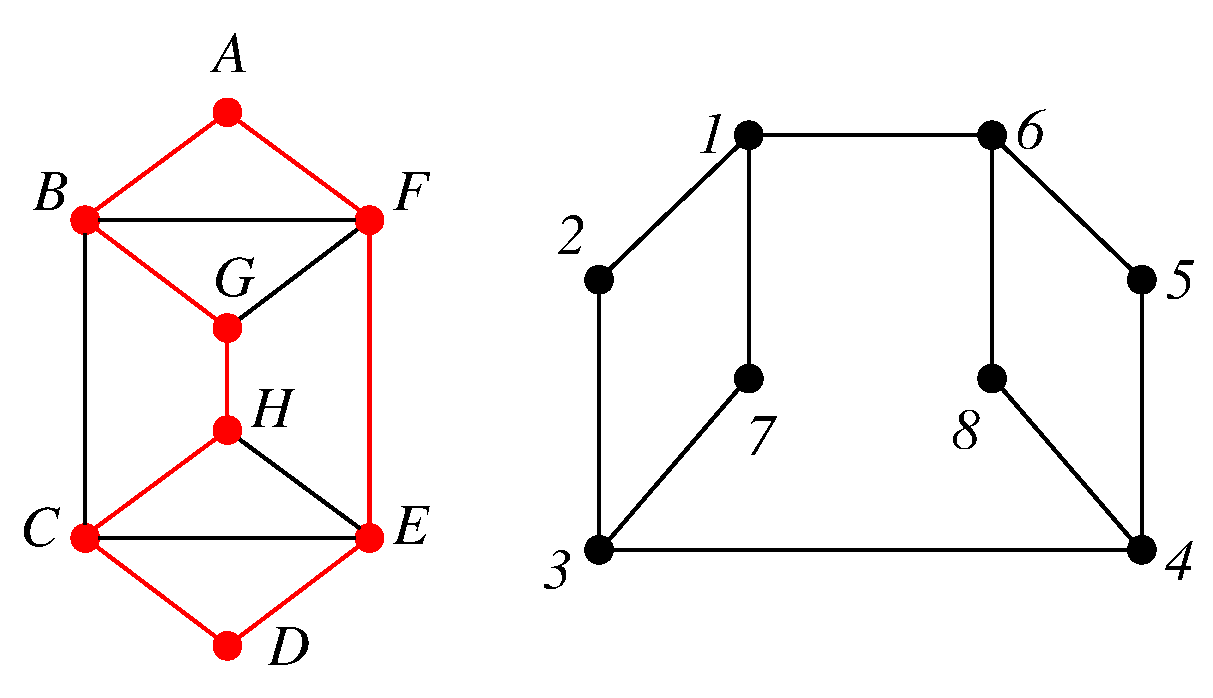
\includegraphics[scale = 0.4]{figures/2-conn-vs-hamilton.pdf}
\caption{Un grafo hamiltoniano (a sinistra, con un ciclo evidenziato) e un grafo 2-connesso (a destra).
Si provi a verificare che quello a destra è effettivamente un grafo 2-connesso
cancellando un vertice qualsiasi}
\end{figure}
\chptr{Alberi}

\section{Alberi e proprietà}

\begin{tcolorbox}[colback=yellow!30, colframe=yellow!30!black, title = {Alberi e Foreste}]
\begin{itemize}
    \item \textbf{Foresta}: un grafo senza cicli.
    \item \textbf{Albero}: un grafo \textit{connesso} e senza cicli.
\end{itemize}
\end{tcolorbox}

\begin{osservaz}
Un grafo è una foresta se e solo se ogni sua componente connessa è un albero.

Sia infatti $G$ un grafo con proprietà di foresta; allora $G$ è un grafo senza
cicli; se $G$ è connesso, allora esso è anche un albero; altrimenti, $G$ è
costituito da più di una componente connessa; essendo $G$ senza cicli per
ipotesi, ogni componente di $G$ deve essere un albero. Si supponga ora che
$G$ sia un grafo connesso con proprietà di albero; $G$ allora non ha cicli
ed è una foresta; sia invece $G$ sconnesso tale per cui ogni componente
sia un albero; allora ogni componente di $G$ (e $G$ stesso) non ha cicli
e quindi è una foresta.
\end{osservaz}

\subsection*{Teorema sugli alberi}
Sia $T=(V,E)$ un grafo non connesso finito. Le seguenti affermazioni
sono equivalenti:
\begin{enumerate}
\item $T$ è un albero.
\item $\forall v,v'\in V, \exists!$ cammino in $T$ che congiunge $v,v'$.
\item \textbf{Minimalità della connessione:}

$T$ è connesso e $\forall e\in E, T-e:=(V,E\setminus \{e\})$ è sconnesso.


\item \textbf{Massimalità rispetto all'assenza di cicli:}

$T$ non ha cicli e $\forall e \in \binom{V}{2}\setminus E, T+e:=(V,E\cup\{e\})$ possiede cicli.
\end{enumerate}

\subsection*{Lemma delle foglie}
Sia $T$ un albero finito avente almeno due vertici. Allora $T$ possiede almeno
due foglie.
$\\\\$
\textit{\textbf{Dimostrazione:}} Sia $\mathcal{P}$ l'insieme di  tutti i cammini
possibili in $T$. Poiché $T$ è finito, $\mathcal{P}$ è finito. Dunque esiste un
cammino $P=(v_0,...,v_k) \in \mathcal{P}$ che abbia lunghezza massima $k$:
\[ k=l(P)\geq l(P') \quad \forall P'\in\mathcal{P} \]
Dimostriamo che $v_0,v_k$ sono due foglie di $T$. Supponiamo che $v_0$ non sia
una foglia. Quindi $\deg_T(v_0)\geq 2$. Sia allora $v'$ vertice del secondo
lato $\{v_0,v'\}$. $v'\not\in\{v_1,...,v_k\}$, perché altrimenti si creerebbero
cicli. Ma allora si otterrebbe una passeggiata $P'=(v',v_0,...,v_k)$ di lunghezza
maggiore di $P$. Quindi necessariamente $\deg_T(v_0)=1$.
\cvd


\begin{osservaz}
Il \textit{Lemma delle foglie} è falso se non si assume che l'albero sia
finito. Esistono alberi infiniti che possiedono una o nessuna foglia
(si prenda come esempio un cammino infinito).
\end{osservaz}


\subsection*{Lemma della rimozione delle foglie (ex 20.8)}
Se $G$ è un grafo connesso e $v$ è una sua foglia, allora $G - v$ è connesso.

\subsection*{Corollario della rimozione delle foglie (ex 20.9)}
Sia $T$ un albero e sia $v$ una sua foglia. Allora $T - v$ è ancora un albero.


\section{\underline{Alberi e formula di Eulero}}

\begin{tcolorbox}[
        enhanced,
        breakable,
        title={Teorema di caratterizzazione degli alberi finiti con formula di Eulero}
    ]
    Sia $T=(V,E)$ un grafo finito. Le seguenti affermazioni sono equivalenti:
    \begin{enumerate}
        \item $T$ è un albero;
        \item $\forall v,v'\in V,\exists! \text{ cammino in} T \text{ che congiunge} v,v'$;
        \item Minimalità della connessione;
        \item Massimalità rispetto all'assenza di cicli;
        \item \textbf{$T$ è connesso e vale la seguente formula di Eulero:}
    \end{enumerate}
    \[ |V|-1=|E| \]
    \textit{\textbf{Dimostrazione:}} Mostriamo che (1) $\Rightarrow$ (5). Procediamo
    per induzione su $|V(T)|$.
    \\\\
    $|V(T)|=1$ (\textbf{base induzione}): $T$ consiste in un vertice isolato, dunque $|V(T)|=1$ e $|E(T)|=0
    \Longrightarrow |V(T)|-1 = 1-1 = 0 = |E(T)|$.
    \\\\
    $|V(T)|\geq 2, |V(T)|-1\Longrightarrow|V(T)|$ (\textbf{passo induttivo}) Sia $T$ un albero con
    almeno 2 vertici. Assumiamo che la formula di Eulero valga su tutti gli alberi che
    possiedono un vertice in meno di $T$ (ipotesi induttiva). Grazie al lemma 20.6, $T$
    possiede almeno due foglie $v,w$. Grazie al \textit{Corollario della rimozione delle foglie},
    $T-v$ è un albero. Segue che $|V(T-v)|=|V(T)|-1$, dunque per ipotesi induttiva vale la formula di
    Eulero per $T-v$:
    \begin{align*}
        |V(T-v)|-1=|E(T-v)| \Longrightarrow 1&+|V(T-v)| - 1 = 1+|E(T-v)|\\
        &\Downarrow\\
        |V(T)|-1&=|E(T)|
    \end{align*}

    Il passo induttivo è verificato, dunque grazie al principio di induzione di prima forma
    l'implicazione (1)$\Rightarrow$(5) è sempre vera.
    \\\\
    Mostriamo ora che (5) $\Rightarrow$ (1). Procediamo per induzione su $|V(T)|$.
    \\\\
    $|V(T)|=1$ (base induzione): $T$ possiede un solo vertice: è un albero e vale (1).
    \\\\
    $|V(T)|\geq 2, |V(T)|-1\Longrightarrow|V(T)|$. Sia $T$ un grafo finito
    connesso con almeno due vertici e che soddisfa la formula di Eulero. Assumiamo che l'implicazione
    (5)$\Rightarrow$(1) sia vera per tutti i grafi finiti connessi con esattamente
    $|V(T)|-1$ vertici e per i quali vale la formula di Eulero (ipotesi induttiva).
    Mostriamo che $T$ ammette almeno una foglia.
    Supponiamo che $T$ non abbia foglie; segue che:
    \begin{align*}
        &\forall w\in V(T)\\
        &\deg_T(w)\not = 0 \text{ per ipotesi sulla connessione e sul numero minimo di vertici}\\
        &\deg_T(w)\not = 1 \text{ per supposizione sull'assenza di foglie}\\
        &\Longrightarrow \deg_T(w)\geq 2
    \end{align*}
    Vale, per ipotesi (vale Eulero per $T$)$^*$ e per la relazione fondamentale dei grafi finiti$^{**}$:
    \[ 2(|V(T)|-1)\stackrel{\text{*}}{=}2|E(T)|\stackrel{\text{**}}{=}\sum_{w\in V(T)}\deg_T(w)\geq \sum_{w\in V(T)}2=2|V(T)| \]
    Il che è assurdo, a causa del fatto che si è assunta l'assenza di foglie.
    Quindi $\exists v$ foglia di $T$. Allora per il \textit{Lemma della rimozione delle foglie}
    $T-v$ è connesso.
    Siccome $T$ soddisfa la formula di Eulero,
    \[ (|V(T)|-1) -1 = |E(T)|-1 \Rightarrow |V(T-v)|-1=|E(T-v)|\]
    quindi $T-v$ soddisfa la formula di Eulero
    e ad esso si può applicare l'ipotesi induttiva: $T-v$ è un albero. $T$ non
    può avere un ciclo, perché tale ciclo dovrebbe attraversare vertici di grado
    maggiore o uguale di 2, dunque non può attraversare la foglia. Ma per ipotesi
    $T-v$ è un albero, dunque tale ciclo non può esistere. Allora $T$ è un albero.
    Il passo induttivo è verificato, quindi l'implicazione inversa è sempre vera
    grazie al principio di induzione di prima forma.
    \cvd
\end{tcolorbox}



\section{\underline{Alberi di copertura}}
\begin{tcolorbox}[colback=yellow!30, colframe=yellow!30!black, title=Albero di copertura]
Sia $G$ un grafo. Un sottografo $T$ di $G$ è un albero di copertura (spannig tree) se:
\begin{itemize}
\item $T$ è un albero.
\item $V(T)=V(G)$
\end{itemize}
\end{tcolorbox}

La Figura \ref{spanning} mostra un grafo $G$ ed evidenzia un suo possibile
spanning tree.

\begin{figure}[H]
\centering
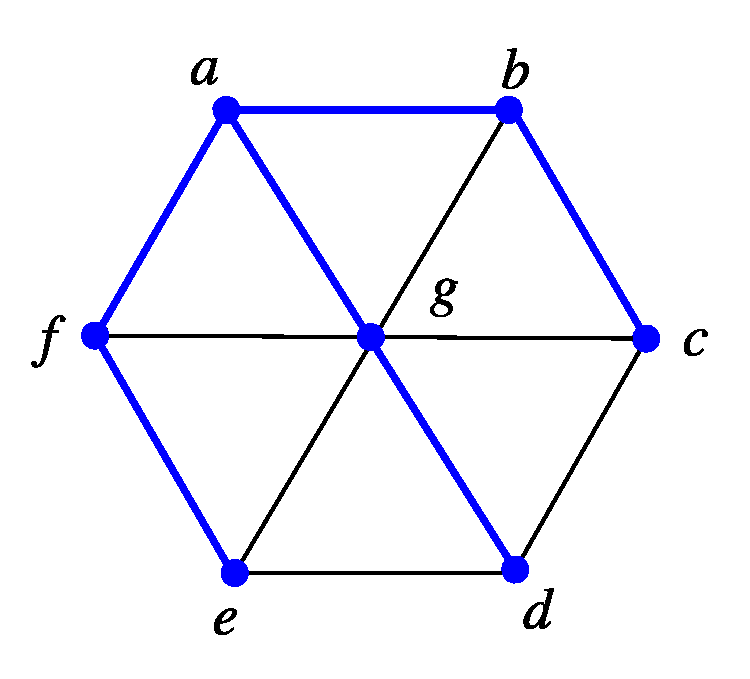
\includegraphics[scale = 0.6]{figures/spanningtree.pdf}
\caption{Grafo $G$ con spanning tree (blu)}
\label{spanning}
\end{figure}

\begin{osservaz}
Se $G$ ammette spanning treee, allora $G$ è connesso. Infatti, se
$T$ è uno spanning tree per $G$, allora $V(T)\subseteq V(G)$ e
$E(T)\subseteq E(G)$. Quindi un cammino in $T$ è anche un cammino
in $G$. Poiché $T$ è connesso (per definizione di albero), allora
lo è anche $G$.
\end{osservaz}

\begin{tcolorbox}[title={Esistenza dell'albero di copertura per grafi connessi finiti}]
Se $G$ è un grafo finito connesso, allora esso ammette un albero di copertura.
$\\\\$
\textit{\textbf{Dimostrazione:}} Sia $G$ un grafo finito e connesso. Definiamo
l'insieme \[ \mathcal{C}:=\{C|C \text{ è un sottografo connesso di } G \text{ e } V(C)=V(G)\} \]
Mostriamo che in $\mathcal{C}$ esiste un albero.
Osserviamo che $\mathcal{C}\not=\varnothing$ perché $G\in\mathcal{C}$ grazie
all'ipotesi iniziale. Definiamo
\[ S:=\{n\in\mathbb{N} | n=|E(C)|, C\in\mathcal{C}\} \subset \mathbb{N} \]
Osserviamo che $|E(G)|\in S\Longrightarrow S\not=\varnothing$. Per il teorema del buon ordinamento dei naturali
\[ \exists m:=\min S \Longrightarrow \exists \overline{C}\in\mathcal{C}: |E(\overline{C})|=m\leq |E(C)| \quad \forall C\in\mathcal{C} \]
Mostriamo che $\overline{C}$ è un albero.
Supponiamo per assurdo che non lo sia. Quindi grazie al teorema 20.4 \[\exists e\in E(\overline{C}):
\overline{C}-e=(V(\overline{C}), E(\overline{C})\setminus\{e\})\in\mathcal{C}\]
Ma allora $|E(\overline{C}-e)| = |E(\overline{C})|-1 \in S$ e
avremmo $|E(\overline{C})|\leq |E(\overline{C})|-1$, che è assurdo.

\cvd
\end{tcolorbox}


\part{Esercizi}

\chptr{Problemi di Insiemistica}

\section{Dimostrazioni per induzione}

A tempo di stesura della presente dispensa, la dimostrazione per induzione
costituisce l'unica tipologia di esercizio appartenente all'ambito degli
insiemi e richiesta frequentemente in sede d'esame.
La dimostrazione per induzione eccelle qualora rispetti tutti i punti qui
sotto elencati:
\begin{enumerate}
\item Dichiarazione della proposizione che si intende dimostrare:
generalmente si tratta della \textit{formuletta} indicizzata su $n$.
Si tratta di un passo essenziale per far comprendere a coloro che
leggono \textit{cosa} intendiamo dimostrare.
\item Dichiarazione dell'insieme entro il quale dimostrare la
validità della proposizione.
\item Verifica della \textbf{base dell'induzione}.
\item Dichiarazione dell'\textbf{ipotesi induttiva} e verifica del
\textbf{passo induttivo} mediante l'ipotesi.
\item Conclusioni: terminare il passo induttivo non basta; di fatto
la conclusione consiste nel constatare che, verificati caso base e
passo induttivo, la validità della proposizione si fonda sul meccanismo
del principio di induzione (bisogna dunque nominarlo).
\end{enumerate}

\begin{tcolorbox}[enhanced, breakable, colback=blue!30, colframe=blue!30!black, title=Esempio]
Si dimostri per induzione su $n\in\mathbb{N}$ che, per ogni intero $n\geq0$,
vale: \[ \sum_{k=0}^{n}4k3^k=3+3^{n+1}(2n-1) \]
\textit{Soluzione (dimostrazione):} si procede per induzione su $n\in\mathbb{N}$,
considerando la proposizione \[P(n):=\left( \sum_{k=0}^{n}4k3^k=3+3^{n+1}(2n-1) \right)\]
\underline{$n=0$ (base dell'induzione)} Si deve verificare $P(0)$,
ovvero che $\sum_{k=0}^{0}4k3^k=3+3^{0+1}(2\cdot0-1)$.
Vale:
\begin{align*}
\sum_{k=0}^{0}4k3^k  &=4\cdot0\cdot3^0=0\\
3+3^{0+1}(2\cdot0-1) &=3+3(-1)=3-3=0
\end{align*}
Segue che $\sum_{k=0}^{0}4k3^k=0=3+3^{0+1}(2\cdot0-1)$, dunque la base
dell'induzione è verificata.

\underline{$n\in\mathbb{N},n\Longrightarrow n+1$ (passo induttivo)}
Si assume ora che l'uguaglianza espressa da $P(n)$ sia vera per
qualche $n\in\mathbb{N}$ (ipotesi induttiva). Si deve mostrare che
vale $P(n+1)$, cioè:
\[ \sum_{k=0}^{n+1}4k3^k=3+3^{(n+1)+1}(2(n+1)-1) \]
Vale:
\begin{align*}
\sum_{k=0}^{n+1}4k3^k &=4(n+1)3^{n+1} + \sum_{k=0}^{n}4k3^k \stackrel{\text{ipotesi induttiva}}{=}\\
                        &=4(n+1)3^{n+1} + 3+3^{n+1}(2n-1) =\\
                        &=3+3^{n+1}(2n-1+4(n+1)) =\\
                        &=3+3^{n+1}(6n+3) =\\
                        &=3+3^{n+1}3(2n+1) =\\
                        &=3+3^{(n+1)+1}(2(n+1)-1)
\end{align*}
Dunque vale $P(n+1)$ e il passo induttivo è verificato. Grazie al
principio di induzione di prima forma, $P(n)$ vale $\forall n\in\mathbb{N}$.
\end{tcolorbox}
\chptr{Problemi di Aritmetica Modulare}

\section{Sistemi di congruenze semplici}
Sistemi di questo genere richiedono l'applicazione del teorema cinese
del resto, la cui dimostrazione fornisce il procedimento per raggiungere la
soluzione. Pertanto i punti essenziali sono:
\begin{enumerate}
\item Identificare e dichiarare l'insieme delle soluzioni.
\item Verificare la compatibilità.
\item Calcolare una soluzione particolare.
\item Costruire l'insieme delle soluzioni.
\end{enumerate}

\begin{tcolorbox}[enhanced, breakable, colback=blue!30, colframe=blue!30!black, title=Esempio]
Si determinino tutte le soluzioni del seguente sistema di congruenze:
\[
\begin{cases}
    x\equiv 100 &\Mod{150}\\
    x\equiv 65  &\Mod{85}
\end{cases}
\]
Si dica inoltre, motivando la risposta, se il precedente sistema una
soluzione divisibile per 2551.
$\\\\$
\textit{Soluzione:} Sia $S\subset\mathbb{Z}$ l'insieme delle soluzioni del sistema di
cui sopra e calcoliamolo. Verifichiamo anzitutto la compatibilità del
sistema. Grazie al teorema cinese del resto vale la relazione
$S\not=\varnothing \Longleftrightarrow (150,85)|100-65$. Calcoliamo
dunque $(150,85)$ tramite fattorizzazione:
\[ 150=2\cdot3\cdot5^2, 85=5\cdot17 \Longrightarrow (150,85)=5 | 100-65=35 \]
Dunque, grazie al teorema cinese del resto, $S\not=\varnothing$. Inoltre
vale: \[ \text{(1) } 100-65=7\cdot5=7(150,85) \]
Calcoliamo una soluzione particolare $c\in S$. Lanciamo l'algoritmo di
Euclide su 150 e 85:
\begin{align*}
150 &=85+65                & 5&=65-3\cdot20 =\\
85  &=65+20                &  &=65-3\cdot(85-65)=4\cdot65-3\cdot85\\
65  &=3\cdot20+\textbf{5}  &  &=4\cdot(150-85)-3\cdot85=4\cdot150-7\cdot85 \Rightarrow\\
20  &=4\cdot5+0            &  &\Rightarrow (150,85)=4\cdot150-7\cdot85 \text{ (2)}
\end{align*}

Grazie alle uguaglianze (1) e (2) vale:
\begin{align*}
    100-65=7\cdot(150,85)&=28\cdot150-49\cdot85\\
    &\Updownarrow\\
    100-28\cdot150&=65-49\cdot85=-4100=:c\in S
\end{align*}

Grazie al teorema cinese del resto, l'insieme delle soluzioni può essere
costruito come segue: \[ S=[-4100]_{[150,85]}\subseteq\mathbb{Z} \qquad\text{ dove }\qquad [150,85]=\frac{150\cdot85}{(150,85)}=2550\]
Dunque:
\[ S=[-4100+2\cdot2550]_{[150,85]}=[1000]_{[2550]}\subseteq\mathbb{Z} \]
Alternativamente, $S=\{1000+2550k\in\mathbb{Z}|k\in\mathbb{Z}\}$.

Per rispondere alla seconda domanda, si può procedere in più modi. Notiamo
che la richiesta è equivalente a determinare se l'insieme delle soluzioni
$F$ del seguente sistema di congruenze è non vuoto:
\[
\begin{cases}
    x\equiv 1000 &\Mod{2550}\\
    x\equiv 0    &\Mod{2551}
\end{cases}
\]
Come prima applichiamo il teorema cinese del resto per verificare la
compatibilità (non è necessario calcolare la soluzione). Osserviamo
che $(2550,2551)=1$, perché 2551 è successivo a 2550. Verifichiamo:
\[ (2550,2551)=1|1000-0=1000 \]
Allora $F\not=\varnothing$ grazie al teorema cinese del
retsto ed esistono soluzioni al primo sistema divisibili
per 2551.
\end{tcolorbox}


\newpage
\section{Congruenze con potenza e metodo RSA}
Queste congruenze sono risolvibili in vari modi. Vedremo solo la soluzione
mediante RSA, che tuttavia non risolve tutte le congruenze con potenza. Il
procedimento generale per risolvere questi esercizi è il seguente:
\begin{enumerate}
\item Dichiarare l'insieme delle soluzioni.
\item Verificare l'applicabilità del metodo RSA.
\item Costruire l'insieme delle soluzioni.
\item Calcolare l'esponente.
\item Calcolare esplicitamente la soluzione, eventualmente ricorrendo
al metodo dell'orbita.
\end{enumerate}

\begin{tcolorbox}[enhanced, breakable, colback=blue!30, colframe=blue!30!black, title=Esempio]
Si determinino tutte le soluzioni della seguente congruenza e si calcoli la
minima soluzione positiva:
\[ x^7\equiv59 \Mod{62} \]
\textit{Soluzione:} Sia $S\subseteq\mathbb{Z}$ l'insieme delle soluzioni della congruenza
di cui sopra e calcoliamolo. Verifichiamo l'applicabilità del metodo
RSA, ovvero controlliamo se valgono le seguenti uguaglianze:
\begin{align*}
(59,62)\stackrel{\text{?}}{=}1:      & \text{ osserviamo che 59 è primo
                                        e } 59\not|62 \text{ dunque
                                        } (59,62)=1.\\
(7,\Phi(62))\stackrel{\text{?}}{=}1: & \text{ applicando la moltiplicatività
                                        della Phi di Eulero: }\\
                                    &\Phi(62)=\Phi(2\cdot31)=\Phi(2)\Phi(31)=(2-1)(31-1)=30\\
                                    & \text{7 è primo e } 7\not|30 \text{ dunque } (7,\Phi(62))=1.
\end{align*}
Il metodo RSA è applicabile. La soluzione può allora essere costruita nel
seguente modo:
\[ S=[59^d]_{62}\subseteq\mathbb{Z} \quad d>0, d\in[7]^{-1}_{\Phi(62)} \]
Calcoliamo $d$. Applichiamo l'algoritmo di Euclide a 7 e $\Phi(62)=30$:
\begin{align*}
30 &=4\cdot7+2                & 1&=7-3\cdot2 =\\
7  &=3\cdot2+\textbf{1}       &  &=7-3\cdot(30-4\cdot7)=\\
2  &=2\cdot1+0                &  &=13\cdot7-3\cdot30
\end{align*}
Vale:
\begin{align*}
    &1=13\cdot7+(-3)\cdot30 \Longrightarrow [1]_{30}=[13\cdot7]_{30}+[-3\cdot30]_{30} \Longrightarrow\\
    &\Longrightarrow [1]_{30}=[13]_{30}[7]_{30} \Longrightarrow [7]^{-1}_{30}=[13]_{30}
\end{align*}
Dunque $d=13$. Calcoliamo esplicitamente la soluzione e, per semplificare i
calcoli, studiamo l'orbita di $[59^k]_{62}, k\in\mathbb{N}\setminus\{0\}$.

\begin{center}
\begin{tabular}{c|l}
    \head{k} & \head{Rappresentante di $[59^k]_{62}$}\\
    \hline
    1        & 59\\
    2        & $59^2=3481=56\cdot62+9\equiv9 \Mod{62}$\\
    3        & $59^3=59^2\cdot59\equiv9\cdot59\equiv 35\Mod{62}$\\
    4        & $59^4=(59^2)^2\equiv9^2\equiv 19 \Mod{62}$\\
    5        & $59^5=59^4\cdot59\equiv19\cdot59\equiv 5\Mod{62}$\\
\end{tabular}
\end{center}

Osserviamo che $[59^5]_{62}=[5]_{62}, [59^3]_{62}=[35]_{62}$, dunque
vale:
\[ [59^{13}]_{62}=[59]^{2\cdot5+3}_{62}=[59^5]^2_{62}[59^3]_{62}=[5^2]_{62}[35]_{62}=[25\cdot35]_{62}=[7]_{62} \]
E la soluzione è:
\[ S=[7]_{62}\subseteq\mathbb{Z} \]
e la minima soluzione positiva corrisponde al rappresentante di $[7]_{62}$
ovvero 7.
\end{tcolorbox}
\chptr{Problemi sui Grafi}


\section{Individuare un isomorfismo}
Consideriamo il problema seguente:
\begin{center}
Dati due o più grafi, si desidera stabilire se sono tra loro isomorfi.
\end{center}
Quando si affronta un problema come questo, spesso torna utile ricorrere
alle proprietà mostrate di seguito.
\begin{tcolorbox}[colback=red!30, colframe=red!30!black, title=Alcune caratteristiche dei grafi isomorfi]
Siano $G,G'$ grafi finiti. Supponiamo $G\cong G'$. Allora:
\begin{enumerate}
\item $\text{Score}(G)=\text{Score}(G')$.
\item $G,G'$ hanno lo stesso numero di componenti connesse.
\item $G$ è 2-connesso $\Longleftrightarrow$ $G'$ è 2-connesso.
\item $G$ è hamiltoniano $\Longleftrightarrow$ $G'$ è hamiltoniano.
\item $G,G'$ hanno lo stesso numero di sottografi che sono $k$-cicli.
\item Sia $f:V\to V'$ un isomorfismo. Sia $v\in V$ tale che $\deg_G(v)=k\in\mathbb{N}$.
Siano $v_1,...,v_k \in V$ adiacenti a $v$. Allora $f(v_1),...,f(v_k)$ sono
adiacenti a $f(v)$: \[\deg_G(v)=\deg_G(f(v)) \quad \deg_G(v_i)=\deg_G(f(v_i)) \quad \forall i \in\{1,...,k\}\]
\end{enumerate}
\end{tcolorbox}

La proprietà (6) potrebbe essere la più complessa da applicare. Intuitivamente,
essa permette di trovare grafi tra loro non isomorfi osservando i gradi
di vertici tra loro adiacenti. Un sempio di applicazione di (6) è presente
in uno degli esercizi di esempio mostrati in questa sezione.
\\\\
Supponiamo di avere $G,G'$ grafi finiti. Per stabilire se sono isomorfi, si
controllano le proprietà da (1) a (6). Se anche una sola è falsa, allora
si può concludere con certezza che $G\not\cong G'$. Altrimenti non si può
ancora dare una risposta: infatti si tratta di condizioni sufficienti ma
non necessarie all'esistenza di isomorfismi. Si prova allora a definire un
isomorfismo "a mano".

\newpage
\begin{tcolorbox}[enhanced, breakable, colback=blue!30, colframe=blue!30!black, title=Esempio]
Siano rispettivamente $G_1, G_2, G_3$ i grafi raffigurati qui sotto.
Si dica, motivando la risposta, quali tra essi sono isomorfi e quali no.
\begin{figure}[H]
\centering
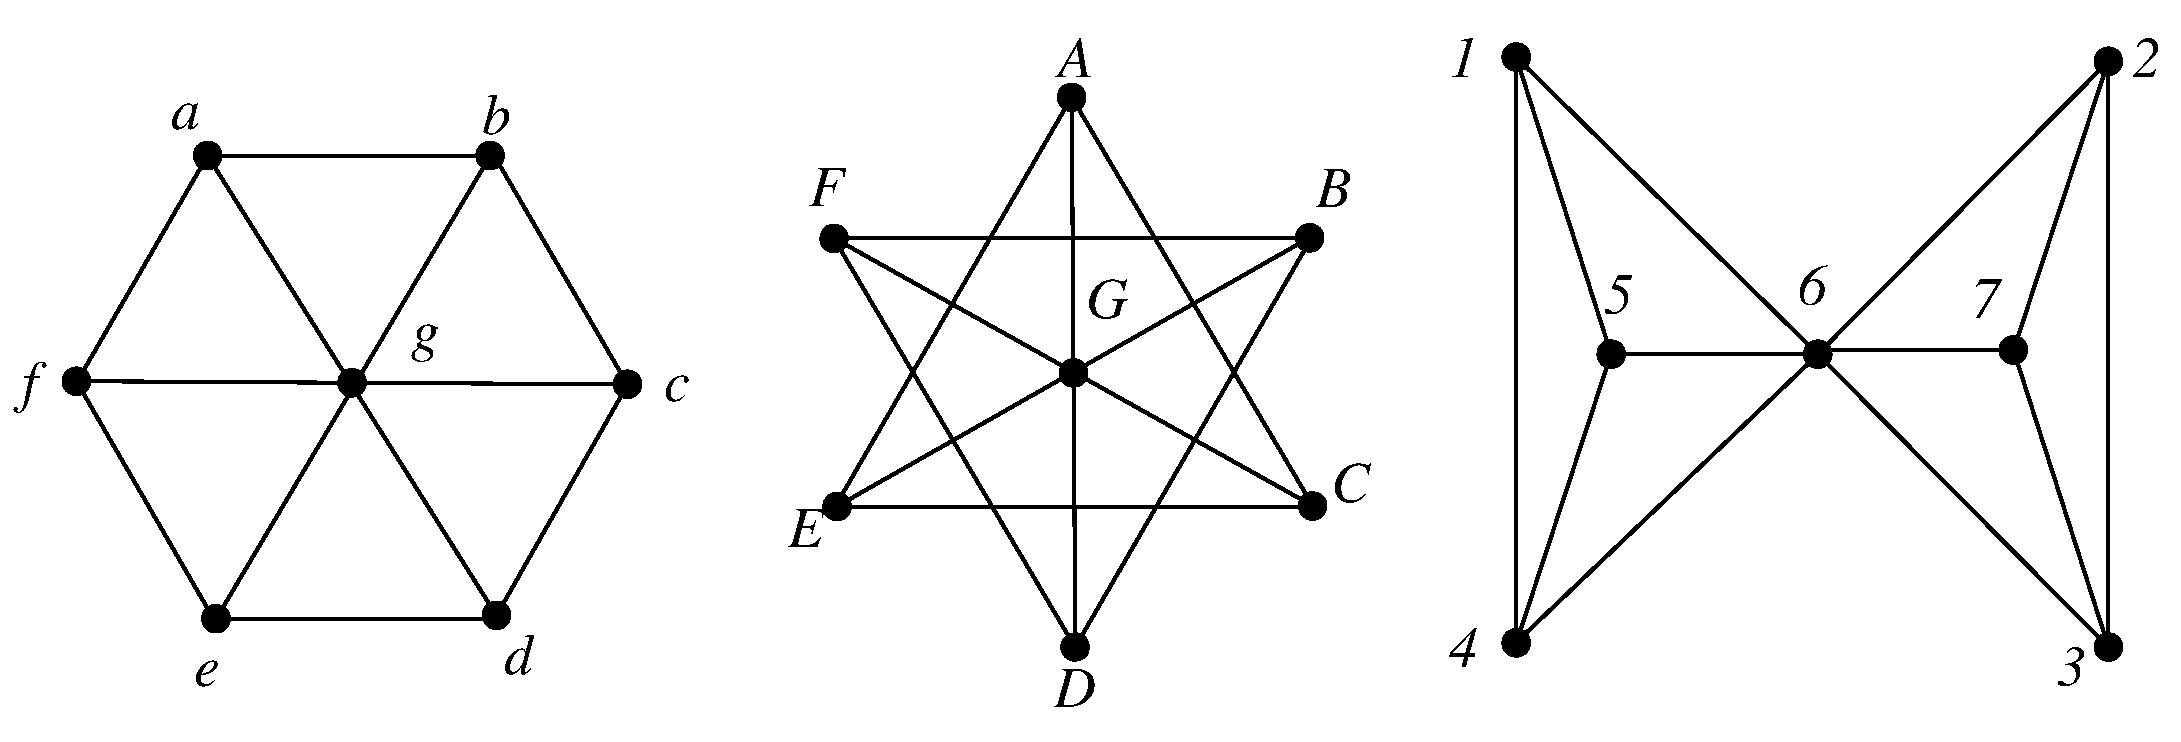
\includegraphics[scale=0.27]{exisomorph.pdf}
\end{figure}
\textit{Soluzione:} verifichiamo prima le condizioni necessarie per l'esistenza
di isomorfismi tra grafi finiti:
\begin{enumerate}
    \item $\text{Score}(G_1) = \text{Score}(G_2) = \text{Score}(G_3)$: nulla si può dire.
    \item In ciascuno dei tre grafi, ogni coppia di vertici può essere collegata con passeggiate. Dunque $G_1,G_2,G_3$ sono connessi: nulla si può dire.
    \item Osserviamo che $(a,b,c,d,e,f,g,a)$ è un ciclo hamoltoniano in $G_1$.
    Dunque $G_1$ è un grafo hamiltoniano e quindi anche 2-connesso. Possiamo inoltre
    notare che $G_2 - G$ e $G_3 - 6$ non sono connessi, quindi $G_2$ e $G_3$ non
    sono grafi 2-connessi. Possiamo concludere che
    \[ G_1 \not\cong G_2 \quad \text{ e } \quad G_1 \not\cong G_3 \]
    \item Dal punto precedente abbiamo concluso che $G_2$ e $G_3$ non sono 2-connessi,
    dunque nemmeno hamiltoniani: nulla si può dire su questi due grafi.
    \item $G_2$ e $G_3$ hanno lo stesso numero di 3-cicli: nulla si può dire.
    \item Notiamo che $G_2$ e $G_3$ hanno un unico vertice di grado massimo:
    $G\in V(G_2)$ e $6 \in V(G_3)$ con $\deg_{G_2}(G) = \deg_{G_3}(6) = 6$.
    Dunque, se esistesse un isomorfismo $f:V(G_2)\to V(G_3)$, allora $f(G) = 6$.
    Osserviamo che $G$ è adiacente a sei vertici, ciascuno di grado 3. D'altra parte,
    anche $6$ è adiacente a sei vertici, ciascuno con grado 3. Non si deduce alcuna
    contraddizione: nulla si può dire.
\end{enumerate}
Non concludendo ancora nulla su $G_2$ e $G_3$, proviamo a definire un isomorfismo
tra questi grafi. Sia:
\begin{align*}
    V(G_2) &\stackrel{f}{\to} V(G_3)\\
    A&\mapsto 2\\
    B&\mapsto 5\\
    C&\mapsto 7\\
    D&\mapsto 4\\
    E&\mapsto 3\\
    F&\mapsto 1\\
    G&\mapsto 6
\end{align*}
Poiché nella colonna di destra appaiono tutti i vertici di $G_3$ senza ripetizioni,
la funzione $f:V(G_2)\to V(G_3)$ è una bigezione. Verifichiamo se si tratta anche
di un morfismo da $G_2$ a $G_3$:
\begin{align*}
    E(G_2) &\stackrel{'f'}{\to}\binom{V(G_3)}{2}\\
    \{A,E\} &\mapsto \{2,3\}\\
    \{A,G\} &\mapsto \{2,6\}\\
    \{A,C\} &\mapsto \{2,7\}\\
    \{E,C\} &\mapsto \{3,7\}\\
    \{E,G\} &\mapsto \{3,6\}\\
    \{C,G\} &\mapsto \{7,6\}\\
    \{F,B\} &\mapsto \{1,5\}\\
    \{F,G\} &\mapsto \{1,6\}\\
    \{F,D\} &\mapsto \{1,4\}\\
    \{D,G\} &\mapsto \{4,6\}\\
    \{D,B\} &\mapsto \{4,5\}\\
    \{B,G\} &\mapsto \{5,6\}\\
\end{align*}
Segue che $f(E(G_2)) \subseteq E(G_3)$, dunque $f$ è un morfismo da $G_2$ a $G_3$.
D'altra parte i lati di $G_3$ che compaiono nella seconda colonna della precedente
lista sono tutti i 12 lati di $G_3$. Allora $f(E(G_2)) = E(G_3)$, ovvero $f$ è un
isomorfismo da $G_2$ a $G_3$. Dunque $G_2 \equiv G_3$.

\end{tcolorbox}



\newpage
\section{Riconoscere uno score}
Si consideri il seguente problema:
\begin{center}
dato $d = (d_1,...,d_n)\in\mathbb{N}^n$, stabilire se esiste un grafo $G$
tale che $\text{Score}(G)=d$
\end{center}
Presentiamo ora un ridottissimo numero di lemmi, o \textit{ostruzioni}, che
consentono di verificare se un vettore di interi può \emph{non} essere lo score
di un grafo. Si sottolinea che:
\begin{itemize}
\item Le ostruzioni sono \textit{condizioni sufficienti ma non
necessarie} all'esistenza di un grafo: dato un vettore $d$, se
anche tutte le ostruzioni mostrate qui fallissero, non
si potrebbe dire alcunché sull'esistenza di un grafo con score
$d$.

\item Alcune ostruzioni non sono applicabili a tutti i vettori:
ciò non implica la non esistenza di un possibile grafo con score
$d$.

\item Queste non sono le uniche ostruzioni esistenti: in base
alle dimensioni e alla conformazione del vettore dato, potrebbero
anzi esistere migliaia di ostruzioni applicabili.
\end{itemize}

\begin{tcolorbox}[colback=red!30, colframe=red!30!black, title=Ostruzione 1]
Sia $d=(d_1,...,d_n)\in\mathbb{N}^n, n\geq1, d_1\leq...\leq d_n$.
\[ d_n > n-1 \Longrightarrow \nexists G:\text{Score}(G)=d \]
\end{tcolorbox}

\begin{tcolorbox}[colback=blue!30, colframe=blue!30!black, title=Esempio: applicazione della prima ostruzione]
Viene dato $d=(1,1,1,2,2,3,4,8)$. Quindi $n=8,d_n=8$
ma $d_n = 8 > n - 1 = 8 - 1 = 7$. Quindi non esiste nessun grafo con
score $d$.
$\\\\$
\textbf{Motivazione:} non può esistere un grafo con tale score,
perché sono previsti $n$ vertici e ognuno di essi può essere
collegato ad al più $n-1$ vertici (ovvero può appartenere ad
al più $n-1$ lati).
\end{tcolorbox}

\begin{tcolorbox}[colback=red!30, colframe=red!30!black, title=Osservazione]
Sia $d=(0,...,0,d_1,...,d_n)\in\mathbb{N}^{n+m}$, dove compaiono
$m$ zeri e vale $0<d_1\leq...\leq d_n$. Sia $d'=(d_1,...,d_n)\in\mathbb{N}^n$.
\[ d \text{ è lo score di un grafo } \Longleftrightarrow d' \text{ è lo score di un grafo} \]
\end{tcolorbox}

\begin{tcolorbox}[colback=blue!30, colframe=blue!30!black, title=Esempio]
Viene dato $d=(0,0,0,1,1,2,2,2,3,4,9)$. L'ostruzione
1 non è verificata, quindi non si può ancora dare una risposta.
Estraiamo da $d$ lo score $d'=(1,1,2,2,2,3,4,9)$ e riapplichiamo
l'ostruzione: $d_n=9>n-1=8-1=7$. Segue che $d'$ non può rappresentare
lo score di un grafo e per l'Osservazione non lo è nemmeno $d$.
\end{tcolorbox}


\begin{tcolorbox}[colback=red!30, colframe=red!30!black, title=Ostruzione 2]
Siano $h,k\in\mathbb{N}\setminus\{0\}$, sia $n:=h+k$ e $d\in\mathbb{N}^n$
tale che $d=(d_1,...,d_h,n-1,...,n-1)$ dove $n-1$ compare $k$ volte
e $d_1\leq...\leq d_h < n-1$.
\[ d_1<k \Longrightarrow \nexists G:\text{Score}(G)=d \]
\end{tcolorbox}
\begin{tcolorbox}[colback=blue!30, colframe=blue!30!black, title=Esempio]
Viene dato $d=(1,2,3,4,5,6,7,8,8)$. L'ostruzione 1
non fornisce informazioni. Notiamo che è applicabile l'ostruzione 2:
$d_1=1<2$ quindi non esistono grafi con score $d$.
\end{tcolorbox}

\noindent Una motivazione verbale esaustiva può essere la seguente:
\emph{non può esistere un grafo con tale score,
perché sarebbero previsti $n$ vertici di cui $k$ collegati a
tutti gli altri, quindi $d_1$ dovrebbe valere almeno $k$.}

\begin{tcolorbox}[colback=blue!30, colframe=blue!30!black, title=Esempio: combinare l'osservazione alle altre ostruzioni]
Viene dato $d=(0,0,0,2,3,3,3,3,3,3,4,10,10,10)$.
\begin{enumerate}
\item $d_n=10 \not> n-1=14-1=13$: l'ostruzione 1 non fornisce
informazioni.

\item Non è applicabile l'ostruzione 2. Però il vettore $d'$
è valido, quindi applichiamo l'osservazione: $d'_1=2<3$, quindi
$d'$ non è lo score di un grafo e pertanto nemmeno $d$.
\end{enumerate}
\end{tcolorbox}  




\begin{tcolorbox}[colback=red!30, colframe=red!30!black, title=Ostruzione 3]
Sia $n\in\mathbb{N},n\geq3$. Sia $d=(d_1,...,d_n)\in\mathbb{N}^n,
d_1\leq...\leq d_n$. Definiamo: $L:=\left|\left\{ i\in\{1,...,n-2\}|d_i\geq2 \right\}\right|$.
\[ L < d_{n-1}+d_n-n \Longrightarrow \nexists G:\text{Score}(G)=d \]
\end{tcolorbox}

\begin{tcolorbox}[colback=blue!30, colframe=blue!30!black, title=Esempi]
Viene dato $d=(1,1,1,3,5,5,7,7,8,8)$.
\begin{enumerate}
\item $d_n=8>n-1=10-1=9$: nulla si può dire.
\item Ostruzione 2 non applicabile.
\item $L=5 < d_n+d_{n-1}-n=8+8-10 = 6 \Longrightarrow \nexists G:\text{Score}(G)=d$.
\end{enumerate}
Viene dato $d=(2,2,2,2,3,3,3,5,6)$.
\begin{enumerate}
\item $d_n=6>n-1=9-1=8$: nulla si può dire.
\item Ostruzione 2 non applicabile.
\item $L=7<5+6-9=2$: nulla si può dire.
\end{enumerate}
\end{tcolorbox}  

\begin{tcolorbox}[colback=red!30, colframe=red!30!black, title=Ostruzione 4]
Si veda il \textbf{lemma delle strette di mano}.
\[ d \text{ non soddisfa il lemma delle strette di mano} \Longrightarrow \nexists G:\text{Score}(G)=d \]
\end{tcolorbox}



\newpage
\section{Il teorema dello score}
Una volta verificato che il vettore fornito non soddisfa alcuna ostruzione,
è possibile procedere con l'applicazione del teorema dello score, che
rappresenta un buon metodo di verifica e costruzione di un possibile grafo
con score dato.
\begin{tcolorbox}[title=Teorema dello Score]
Sia $n\geq2$ e sia $d=(d_1,...,d_n)\in\mathbb{N}^n$ tale che $d_1\leq...\leq d_n\leq n-1$.
Definiamo $d'=(d'_1,...,d'_{n-1})\in\mathbb{N}^{n-1}$ ponendo:
\begin{align*}
d'_i:=
\begin{cases}
    d_i   & i<n-d_n\\
    d_i-1 & i\geq n-d_n
\end{cases}
\end{align*}
Allora $d$ è lo score di un grafo se e solo se lo è $d'$.
\end{tcolorbox}

\noindent Si noti che il teorema dello score incorpora già in sé la condizione
dell'ostruzione 1. La proprietà più apprezzabile di questo teorema
risiede nel fatto che esso fornisce un algoritmo che abbassa la
complessità dello score fornito, riducendolo ad una serie di casi
possibili trattabili con molta facilità. Il lemma seguente ci mostra
quali sono questi casi.

\begin{tcolorbox}[enhanced, breakable, colback=red!30, colframe=red!30!black, title={Casi notevoli dopo l'applicazione del teorema dello score}]
Sia $n\in\mathbb{N}\setminus\{0\}$ e sia $d=(d_1,...,d_n)\in\mathbb{N}^n$
tale che $d_1\leq...\leq d_n\leq 2$. Valgono:
\begin{enumerate}
\item Se $d=(0,...,0,2)$ oppure $n\geq 2$ e $d=(0,...,0,2,2)$ allora
non esiste un grafo con score $d$.

\item Se $d=(0,...,0)$ o $d=(0,...,0,2,2,...,2)$ ($m\geq 3$ elementi
di grado 2) allora esiste un grafo con tali score: $G_1$ con tutti
i vertici isolati, $G_2$ con $n-m$ vertici isolati e un $m$-ciclo.

\item Supponiamo che compaia almeno una volta l'unità 1. Se il numero
di volte in cui compare 1 è dispari, allora non esiste $G$ con tale
score (conseguenza del lemma delle strette di mano).

\item Supponiamo che 1 compaia in numero pari $2k+2\geq 2$ ($k\geq 0$),
che il numero di 0 sia $h\geq0$ e i 2 in numero $m\geq0$:
\[ d=(0,...,0,1,1,...,1,1,2,...,2) \]
Allora il seguente grafo $G$ ha score $d$:
\begin{figure}[H]
\centering
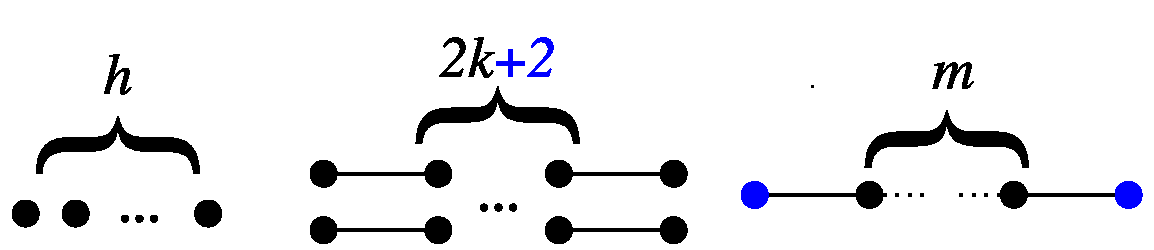
\includegraphics[scale=0.4]{base.pdf}    
\end{figure}
\end{enumerate}
\end{tcolorbox}


\begin{tcolorbox}[enhanced, breakable, colback=blue!30, colframe=blue!30!black, title={Esempio di applicazione del teorema dello score}]
Stabilire se esiste un grafo con score $d=(2,2,2,2,3,3,3,5,6)$. In caso affermativo,
costruire un possibile grafo con score $d$, mediante il teorema dello score.
$\\\\$
\textit{Soluzione:} Passiamo in rassegna le ostruzioni viste finora:
\begin{enumerate}
    \item Osserviamo che $6>9-1$: nulla si può dire.
    \item Questa ostruzione non è applicabile: nulla si può dire.
    \item $L=7<5+6-9 = 2$: nulla si può dire.
    \item $d$ soddisfa il lemma dell strette di mano: nulla si può dire.
\end{enumerate}
Non avendo concluso nulla, ricorriamo al teorema dello score (sappiamo già dall'ostruzione 1
che il teorema è applicabile a $d$).
\begin{center}
    \begin{tabular}{c|lllllllll}
        $d$   & 2 & 2 & \textcolor{white}{2} & \textcolor{white}{2} & \textcolor{white}{3} & \textcolor{white}{3} & \textcolor{white}{3} & \textcolor{white}{5} & \textcolor{yellow}{6}\\
        \hline
        $d'$  & 2 & 2 & 1 & 1 & 2 & 2 & 2 & 4 & $\times$\\
              & 1 & 1 & 2 & \textcolor{white}{2} & \textcolor{white}{2} & \textcolor{white}{2} & \textcolor{white}{2} & \textcolor{green}{4} & \tiny{ordinato}\\
        \hline
        $d''$ & 1 & 1 & 2 & 1 & 1 & 1 & 1 & $\times$ &\\
              & 1 & 1 & 1 & 1 & \textcolor{red}{1} & \textcolor{red}{1} & \textcolor{red}{2} & & \tiny{ordinato}
    \end{tabular}
\end{center}
Ci siamo ricondotti ad una forma notevole dello score, facilmente
rappresentabile. Costruiamo $G''$, che ha score $d''$:
\begin{figure}[H]
\centering
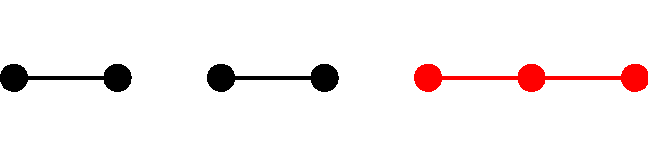
\includegraphics[scale=0.4]{basescore.pdf}    
\end{figure}
Per il teorema dello score, sono score di qualche grafo anche $d'$ e
$d$. Costruiamo un grafo $G$ con score $d$ mediante il teorema dello score:
\begin{figure}[H]
\centering
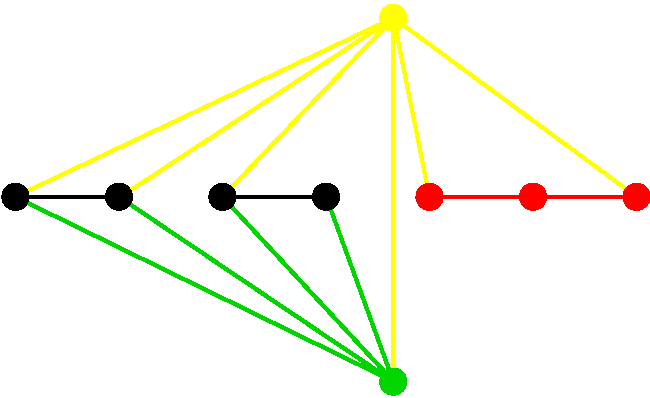
\includegraphics[scale=0.4]{teoscore.pdf}
\end{figure}
\end{tcolorbox}

\noindent Sottolineamo alcuni punti:
\begin{itemize}
    \item Il grafo $G$ finale potrebbe non essere l'unico con score $d$ (potrebbero esistere alternative nella costruzione del grafo).
    \item Sono stati omessi i nomi dei vertici, ma è buona prassi indicarli sempre, in particolare all'esame.
\end{itemize}



\section{Altri problemi sullo score}
Appurato che un vettore $d$ è lo score di un grafo, si potrebbe
estendere ulteriormente il problema chiedendosi se esistono
grafi con score $d$ che sono connessi o sconnessi, hamiltoniani,
2-connessi o aventi un certo numero di componenti connesse.

\subsection*{Connessione e sconnessione}
\begin{tcolorbox}[colback=red!30, colframe=red!30!black, title=Forzatura alla connessione]
Sia $G=(V,E)$ un grafo  finito e sia $n=|V|$ il numero
di vertici di $G$. Siano $m:=\min\{\deg_G(v)|v\in V\},
M:=\min\{\deg_G(v)|v\in V\}$. Vale:
\[ m\geq n-M-1 \Longrightarrow G \text{ è connesso} \]
In termini di score, se viene fonrnito $d=(d_1,...,d_n)\in\mathbb{N}^n:
n\geq1, d_1\leq...\leq d_n$, per i grafi con tale score, se
esistono, vale:
\[ d_1+d_n \geq n-1 \Longrightarrow G\text{ connesso }\forall G:\text{Score}(G)=d \]
\end{tcolorbox}
\begin{osservaz}
La forzatura alla connessione è verificabile
anche attraverso l'Ostruzione 2. Se infatti compaiono vertici di grado
$n-1$, ovvero adiacenti a tutti gli altri, necessariamente tutti i
grafi con score $d$, se esistono, sono connessi.
\end{osservaz}

\begin{tcolorbox}[colback=red!30, colframe=red!30!black, title=Forzatura alla sconnessione]
Sia $G=(V,E)$ un grafo finito. Vale:
\[ |E|<|V|-1 \Longrightarrow G \text{ è sconnesso} \]
In termini di score (si consideri il vettore come sopra):
\[ \frac12\sum_{i=1}^{n}d_i < n-1 \Longrightarrow G\text{ sconnesso } \forall G:\text{Score}(G)=d \]
\end{tcolorbox}
\begin{osservaz}
Se entrambe le forzature falliscono, nulla si può dire sullo score $d$ fornito.
\end{osservaz}

\subsection*{Individuare grafi 2-connessi e hamiltoniani}
\noindent Dalla sezione sui grafi 2-connessi e hamiltoniani, sappiamo che tali
grafi:
\begin{itemize}
\item Non possono contenere foglie.
\item Sono connessi.
\end{itemize}
Vettori contenenti entrate nulle o corrispondenti a 1 sicuramente
non possono essere score di grafi 2-connessi o hamiltoniani.
Il problema del ciclo hamiltoniano è \textit{NP-completo}. In altre
parole, non esistono metodi efficienti per capire se un dato grafo
è hamiltoniano o meno, se non in casi particolari come quelli appena
elencati.





\section{Alberi e score}
Dal teorema di caratterizzazione degli alberi finiti mediante la formula
di Eulero, applicando la relazione fondamentale dei grafi finiti, si può
formulare un utile corollario che lega score e alberi.

\begin{tcolorbox}[colback=green!30, colframe=green!30!black, title={Esistenza di alberi con score dato}]
    Sia $n\geq 2$ e sia $d=(d_1,...,d_n)\in\mathbb{N}^n$ tale che $1\leq d_1\leq...\leq d_n$.
    Allora eisste un albero con score $d$ se e solo se vale la seguente \[ n-1 = \frac12\sum_{i=1}^{n}d_i \]
\end{tcolorbox}
In particolare, affinché un vettore $d$ sia lo score di qualche albero, è importante ricordare questi punti:
\begin{itemize}
    \item Se $d$ ha almeno due entrate, le prime due devono essere pari a 1 (l'albero deve possedere almeno due foglie).
    \item $d$ deve soddisfare la formula di Eulero.
\end{itemize}
In generale, a meno che non ci si imbatta nel vettore $d=(0)$ (è un albero
che consiste in un solo vertice isolato), applicando il corollario appena
visto ad un $d=(\textcolor{blue}{1},\textcolor{blue}{1},...,\textcolor{red}{1},...,d_n)$
di dimensione $n\geq2$,
e supponendo che tutte le entrate cosentano a $d$ di essere uno score di
qualche albero si può facilmente costruire un albero
\begin{enumerate}
    \item creando un cammino di lunghezza $k$, dove $k$ è il numero di entrate
    in $d$ maggiori di $1$;
    \item aggiungendo opportunamente le foglie ai vertici del cammino, secondo
    il loro grado.
\end{enumerate}
\begin{figure}[H]
\centering
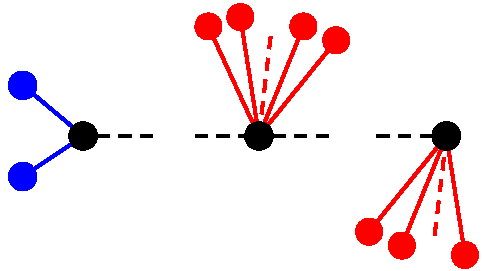
\includegraphics[scale=0.47]{buildtree.pdf}
\caption{\footnotesize Un generico albero $A$ costruito da $d$. Le foglie blu ricordano che $A$ deve contenere almeno due foglie; il cammino iniziale, lungo $k$, è in nero; le foglie rimanenti sono rosse.}
\end{figure}


\section{Un esercizio d'esame sullo score: dall'inizio alla fine}
Si dica, motivando la risposta, quale dei seguenti
vettori è lo score di un grafo e, in caso affermativo,
si costruisca un tale grafo utilizzando il teorema dello score.
\[ d_1=(3,4,4,5,5,5,5,5) \qquad d_2=(2,3,3,3,3,4,5,7,7,7,12,12,12) \]
Si dica inoltre se
\begin{enumerate}
    \item esiste un tale grafo che sia un albero;
    \item esiste un tale grafo che sia hamiltoniano;
    \item esiste un tale grafo che sia sconnesso.
\end{enumerate}
\textit{Soluzione:} non esiste alcun grafo $G$ che
abbia score $d_2$. Infatti, $d_2$ imporrebbe a $G$
di avere 13 vertici dei quali tre di grado 12,
dunque adiacenti a tutti gli altri vertici; allora
il vertice di grado minimo in $G$ dovrebbe avere
almeno grado 3, ma questo contraddice quanto
previsto in $d_2$, dove l'entrata minima equivale
a 2.

Non avendo trovato ostruzioni all'esistenza di
grafi con score $d_1$, procediamo applicando il
teorema dello score a $d_1$. Ciò è possibile
dal momento che $d_{1_8} = 5 \leq 8 - 1$.

\begin{center}
    \begin{tabular}{c|llllllll}
        $d_1$   & 3 & 4 & 4 & 5 & 5 & 5 & 5 & \textcolor{blue}{5}\\
        \hline
        $d_1'$  & 3 & 3 & 4 & 4 & 4 & 4 & \textcolor{orange}{4} & $\times$\\
        \hline
        $d_1''$ & 3 & 3 & 3 & 3 & 3 & \textcolor{red}{3} & $\times$ &\\
        \hline
        $d_1'''$ & 2 & 2 & 2 & 3 & \textcolor{green}{3} & $\times$ &&\\
        \hline
        $d_1''''$ & 1 & 1 & 2 & 2 & $\times$ &&&
    \end{tabular}
\end{center}
Notiamo che da $d_1''''$ è possibile costruire un possibile rispettivo
grafo $G''''$ mostrato di seguito:
\begin{figure}[H]
\centering
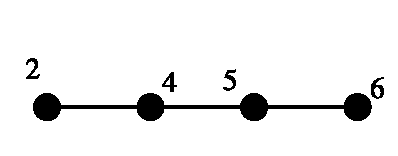
\includegraphics[scale=0.65]{bassefinal.pdf}
\end{figure}

\noindent Per il teorema dello score, allora anche tutti gli altri vettori,
incluso $d_1$, sono lo score di qualche grafo. Costruiamo un grafo
$G$ (si veda la Figura \ref{final}) con score $d_1$ mediante il teorema dello score.
\begin{figure}[H]
\centering
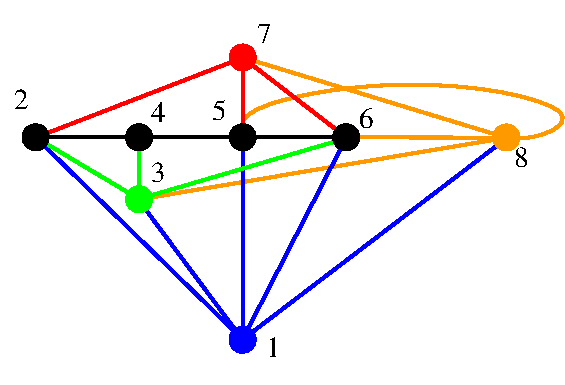
\includegraphics[scale=0.65]{build.pdf}
\caption{$G$}
\label{final}
\end{figure}

\noindent Rispondiamo ora agli altri quesiti:
\begin{enumerate}
    \item Osserviamo che $d_1$ non soddisfa la formula di Eulero:
    \[ 8-1 = 7 \not= \frac{3+4+4+5+5+5+5+5}{2} = 18 \]
    pertanto non esistono alberi con score $d_1$. D'altra parte
    $d_1$, che contiene $8\geq2$ elementi, non possiede nessuna
    entrata pari a 1, ovvero non possiede almeno 2 foglie
    (condizione necessaria all'esistenza di un albero).
    \item Si noti che il ciclo $c=(1,2,3,4,5,6,7,8)$, evidenziato in
    Figura \ref{lasthamiltonian}, in $G$ è hamiltoniano.
    \begin{figure}[H]
    \centering
    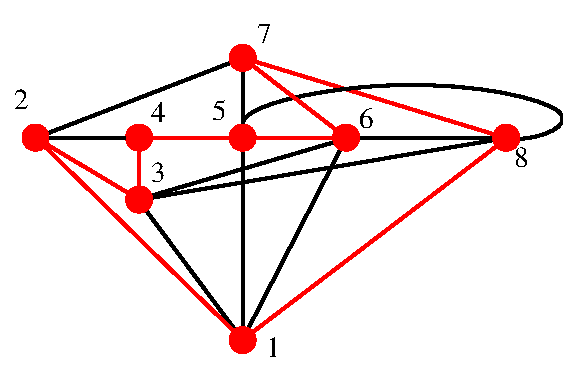
\includegraphics[scale=0.65]{lasthamiltonian.pdf}
    \caption{Un ciclo ($c$) hamiltoniano in $G$.}
    \label{lasthamiltonian}
    \end{figure}
    dunque $G$ è un grafo hamiltoniano con score $d_1$.

    \item Applicando la condizione di \textit{forzatura alla connessione}
    giungiamo alla seguente conclusione:
    \[ 5+3 = 8 > 7 = 8-1 \]
    che soddisfa la forzatura; ma allora ogni grafo con score
    $d_1$ è necessariamente connesso e pertanto non esistono
    grafi sconnessi con score $d_1$.
\end{enumerate}

\part{Appendici}

\chptr{Simbologia}

\begin{align*}
    &\textbf{Simbolo} &\textbf{Significato}                     &&\textbf{Esempio}\\
    &\in              &\text{Appartiene a}                      &&x \in A\\
    &\ni              &\text{Contiene}                          &&A \ni x\\
    &\forall          &\text{per ogni}                          &&\forall x, x = x\\
    &\exists          &\text{esiste (almeno un)}                &&\exists n\in\mathbb{N}: n = 0\\
    &\varnothing      &\text{Insieme vuoto}                     &&\\
    &\subset\text{\footnotemark} &\text{Sottoinsieme di}        && A \subset B\\
    &\subseteq        &\text{Sottoinsieme di}                   &&\\
    &\subsetneq       &\text{Sottoinsieme proprio di}           &&\\
    &\subsetneqq      &\text{Sottoinsieme proprio di}           &&\\
    &:                &\text{Tale che (affermazioni)}           && \exists k\in\mathbb{N}:k=0\\
    &\text{ }|        &\text{Tale che (assioma di separazione)} && \{n|n\in\mathbb{N}, n \text{ è pari}\}
\end{align*}

\footnotetext{La letteratura è ambigua riguardo il significato preciso di questo simbolo. Si consiglia l'utilizzo di altre notazioni più esplicite.}

\end{document}